% Solemtrix · GigaHack 2026 · Vineyard AI Field Challenge (Sireț3) — 5 min pitch + Q&A backup.
% Build: see README.md (xelatex twice). Every number comes from run rc10f / post run 20260927T0452-post-rc10f,
% README.md §6 and §10, src/AI/reports/nn_ablation.md and metrics/route_baseline.json.
\RequirePackage{fix-cm}
\documentclass[aspectratio=169, 11pt, t]{beamer}
\usetheme{solemtrix}
\graphicspath{{img/}{robot/}}

\title[From 311 drone tiles to a 14 km walk]{From 311 drone tiles\\to a 14 km inspection walk}
\subtitle{Classical computer vision first, deep learning only where it pays}
\author[Team Solemtrix]{Team Solemtrix}
\institute[GigaHack 2026]{GigaHack 2026 · Vineyard AI Field Challenge · Sireț3}
\date[27.09.2026]{27 September 2026}

\begin{document}

% ================================================================== 1 · title
\begin{frame}[c]
  \titlepage
\end{frame}

\section{Problem and approach}

% ================================================================== 2 · challenge
\begin{frame}{The challenge: 81.5 ha, one plant at a time}
  \begin{columns}[T]
    \begin{column}{0.33\textwidth}
      \sximg{\linewidth}{overview.jpg}
    \end{column}
    \begin{column}{0.63\textwidth}
      \footnotesize
      \textbf{Input.} 311 GeoTIFF tiles at 2.5\,cm/px (385\,MB) over a 2\,km strip of vineyards,
      orchards, meadows and village yards.
      \vspace{1mm}

      \textbf{Output, 85\,\% scored on objective metrics:}
      \begin{itemize}\setlength{\itemsep}{0.3mm}\scriptsize
        \item canopies, row axes, inter-rows, attributes and waste in Marcaj;
        \item measurements linked by \texttt{vineyard\_id} / \texttt{row\_id};
        \item one closed walking route through every problem spot;
        \item a web map that shows all of it.
      \end{itemize}
      \vspace{1.5mm}
      \begin{sxcard}{The real difficulty}
        Seeing one vine is easy. Seeing 13\,702 the same way, telling them from young orchards and grass,
        then walking only to the ones that matter: that is the problem.
      \end{sxcard}
    \end{column}
  \end{columns}
\end{frame}

% ================================================================== 3 · architecture
\begin{frame}{One offline pipeline, every stage timed}
  \centering
  \begin{tikzpicture}[
      box/.style={draw=sxIndigo200, fill=white, rounded corners=3pt, line width=0.6pt, font=\tiny,
                  minimum height=17mm, align=center, inner sep=1.2mm, text width=20.5mm},
      hot/.style={box, fill=sxIndigo, draw=sxIndigo, text=white},
      human/.style={box, draw=sxAmber, dashed},
      arr/.style={-{Stealth[length=2mm]}, line width=0.9pt, sxIndigo}]
    \node[box]   (in)  {{\scriptsize\bfseries Tiles}\\[0.8mm] 5 ZIPs, 311 GeoTIFF\\ingest + sha256};
    \node[hot, right=5mm of in]  (per) {{\scriptsize\bfseries Perception}\\[0.8mm] rows, canopy\\inter-rows, attributes\\waste, QA previews};
    \node[human, right=5mm of per] (mc) {{\scriptsize\bfseries Marcaj}\\[0.8mm] 5 validated CVAT ZIPs\\human correction\\export};
    \node[hot, right=5mm of mc]  (post) {{\scriptsize\bfseries Post}\\[0.8mm] targets, walking graph\\GTSP route, measure\\farms, roads};
    \node[box, right=5mm of post] (out) {{\scriptsize\bfseries Deliverables}\\[0.8mm] route.geojson\\measurements.csv\\targets, web bundle};
    \foreach \a/\b in {in/per, per/mc, mc/post, post/out} \draw[arr] (\a) -- (\b);
    \node[below=1mm of mc, font=\tiny, text=sxAmber] {human in the loop};
  \end{tikzpicture}

  \vspace{5mm}
  \begin{columns}[T]
    \begin{column}{0.235\textwidth}\begin{sxcard}{Per tile, parallel}8 CPU workers; tiles never wait for each other.\end{sxcard}\end{column}
    \begin{column}{0.235\textwidth}\begin{sxcard}{Cached by config hash}Re-runs reuse per-tile caches; a new config never reads stale ones.\end{sxcard}\end{column}
    \begin{column}{0.235\textwidth}\begin{sxcard}{One source of truth}Every threshold lives in \texttt{default.yaml}.\end{sxcard}\end{column}
    \begin{column}{0.235\textwidth}\begin{sxcard}{Observable}Each run writes its config, a JSONL log and stage timings.\end{sxcard}\end{column}
  \end{columns}
\end{frame}

\section{Perception: computer vision first}

% ================================================================== 4 · efficiency
\begin{frame}{Why computer vision first, deep learning second}
  \begin{columns}[T]
    \begin{column}{0.55\textwidth}
      {\scriptsize\bfseries\color{sxNight} Canopy score on the organisers' 2 example tiles (the only labelled data)\par}
      \vspace{1.5mm}
      \begin{tikzpicture}[x=55mm, y=3.0mm]
        \foreach \lab/\val/\col [count=\i] in {
            {CV: vegetation $\cap$ row corridor}/0.816/sxIndigo,
            {CV $\cup$ U-Net}/0.773/sxGreyBar,
            {CV $\wedge$ U-Net}/0.707/sxGreyBar,
            {U-Net $\cap$ row corridor}/0.675/sxGreyBar,
            {U-Net alone}/0.641/sxGreyBar}{
          \fill[\col, rounded corners=1.5pt] (0,-2*\i) rectangle (\val,-2*\i+0.9);
          \node[anchor=south west, font=\tiny, text=sxMuted, inner sep=0.5pt] at (0,-2*\i+0.95) {\lab};
          \node[anchor=west, font=\scriptsize\bfseries, text=sxNight] at (\val,-2*\i+0.45) {\val};
        }
      \end{tikzpicture}
      \vspace{1mm}

      {\tiny\color{sxMuted} On this small sample the U-Net brings no gain, yet it costs training data and a GPU.
      So it runs only where CV is blind: old vines in grass, 88 tiles, 12.9\,s.\par}
      \vspace{2.5mm}
      {\color{sxIndigo}\footnotesize\bfseries Vines are periodic: structure is a stronger prior than pixels, and almost free to compute.\par}
    \end{column}
    \begin{column}{0.41\textwidth}
      \sxstat{$\approx$\,3 min}{all 311 tiles on a laptop CPU (measured)}
      \vspace{2.5mm}

      \sxstat{0 labels}{no training set; thresholds set on the 2 example tiles}
      \vspace{2.5mm}

      \sxstat{$\approx$\,18 h}{SAM 3 on every tile (extrapolated)}
    \end{column}
  \end{columns}
\end{frame}

% ================================================================== 5 · rows
\begin{frame}{Rows are a 1-D signal, not a 2-D image\sxscore{Axes}{15}}
  \begin{columns}[T]
    \begin{column}{0.3\textwidth}
      \sximg{0.86\linewidth}{rows_preview.jpg}\par\vspace{0.8mm}
      {\tiny\color{sxGrey} Tile r006\_c004: row axes and IDs.\par}
      \vspace{1.5mm}
      \begin{columns}[T, totalwidth=\linewidth]
        \begin{column}{0.48\linewidth}\sxstatsm{674}{rows, 47.7\,km of axes (whole survey)}\end{column}
        \begin{column}{0.48\linewidth}\sxstatsm{44}{blocks, one ID per row across tiles}\end{column}
      \end{columns}
    \end{column}
    \begin{column}{0.66\textwidth}
      \sxstep{1}{Dominant angle, coarse to fine.}{2°, then 0.5° steps: about 100 evaluations instead of 360.}
      \sxstep{2}{Project onto the row normal.}{A 1-D profile: autocorrelation gives the spacing (1.8--3.8\,m), and an SNR $\geq$ 3 rejects orchards.}
      \sxstep{3}{One robust line per peak.}{Huber fit; union-find joins rows across tiles, one ID per row.}
      \vspace{0.5mm}
      \begin{sxcard}{4 \quad Find once, propagate}
        A tile with no confident row is searched again at its neighbours' lattice (angle $\pm$2°, spacing $\pm$15\,\%).
      \end{sxcard}
      \par\vspace{1.5mm}
      \begin{sxexample}
        \sxm{1.00}{row F1 (51/51 rows)}\hfill
        \sxm{1.00}{grouping F1}\hfill
        \sxm{0.05\,\%}{row-length error}
      \end{sxexample}
    \end{column}
  \end{columns}
\end{frame}

% ================================================================== 6 · canopies
\begin{frame}{One polygon per plant, inside its row\sxscore{Canopies}{25}}
  \begin{columns}[T]
    \begin{column}{0.3\textwidth}
      \sximg{\linewidth}{canopy_zoom.jpg}\par\vspace{0.8mm}
      {\tiny\color{sxGrey} Green: canopy. Red: row axis. The grass on the left stays out.\par}
      \vspace{1.5mm}
      \begin{columns}[T, totalwidth=\linewidth]
        \begin{column}{0.52\linewidth}\sxstatsm{13\,702}{plants, whole survey}\end{column}
        \begin{column}{0.44\linewidth}\sxstatsm{149}{disrupted rows}\end{column}
      \end{columns}
    \end{column}
    \begin{column}{0.66\textwidth}
      \sxstep{1}{One colour channel.}{A threshold on Lab a*: no training, no GPU.}
      \sxstep{2}{Only inside the row corridor.}{Grass between rows never becomes canopy.}
      \sxstep{3}{One polygon per plant.}{Connected components: 13\,702 plants, 1.54\,ha of canopy.}
      \sxstep{4}{Attributes from geometry.}{A gap $\geq$ 5\,m marks a row \emph{disrupted}; inter-row cover comes from the vegetation fraction.}
      \vspace{1mm}
      \begin{sxexample}
        \sxm{0.876}{canopy score (official metric)}\hfill
        \sxm{0.856}{canopy IoU}\hfill
        \sxm{0.905}{canopy F1 (0.945 on tile r006\_c004)}\\[1.2mm]
        \sxm{0.960}{inter-row IoU; inter-row F1 1.00 (49/49)}\hfill
        \sxm{1.00}{attributes: row structure 51/51, inter-row cover 49/49}\hfill
        \sxm{585/650}{reference plants matched}
      \end{sxexample}
    \end{column}
  \end{columns}
\end{frame}

% ================================================================== 7 · waste
\begin{frame}{Waste: from cheap filters to big models\sxscore{Waste}{10}}
  \centering
  \begin{tikzpicture}[
      st/.style={rounded corners=3pt, minimum height=14mm, align=center, text width=20mm, inner sep=1.2mm, font=\tiny},
      arr/.style={-{Stealth[length=2mm]}, line width=0.9pt, sxIndigo}]
    \node[st, fill=sxIndigo50]                      (a) {{\small\bfseries 1\,331}\\[0.5mm] rule candidates:\\colour, shape, lattice};
    \node[st, fill=sxIndigo100, right=4.5mm of a]   (b) {{\scriptsize\bfseries OpenCLIP probe}\\[0.5mm] ranks them; trained\\on 11\,292 crops};
    \node[st, fill=sxIndigo200, right=4.5mm of b]   (c) {{\scriptsize\bfseries SAM 3}\\[0.5mm] verifies the top crops;\\13\,s each, so few};
    \node[st, fill=sxIndigoLight, text=white, right=4.5mm of c] (d) {{\scriptsize\bfseries Team}\\[0.5mm] approves every box\\before export};
    \node[st, fill=sxIndigo, text=white, right=4.5mm of d] (e) {{\small\bfseries 11}\\[0.5mm] waste boxes\\exported};
    \foreach \x/\y in {a/b, b/c, c/d, d/e} \draw[arr] (\x) -- (\y);
  \end{tikzpicture}

  \vspace{5mm}
  \begin{columns}[T]
    \begin{column}{0.5\textwidth}
      \centering
      \sximg{19mm}{waste_ok1.jpg}\hspace{1.5mm}\sximg{19mm}{waste_ok2.jpg}\hspace{1.5mm}\sximg{19mm}{waste_rej.jpg}\\[0.8mm]
      {\tiny\color{sxMuted}\makebox[19mm]{exported}\hspace{1.5mm}\makebox[19mm]{exported}\hspace{1.5mm}\makebox[19mm]{rejected}\par}
    \end{column}
    \begin{column}{0.46\textwidth}
      \footnotesize
      Each stage is more expensive and sees fewer crops.\\[2mm]
      \textbf{Precision over recall:} nothing reaches Marcaj without an approval, so false boxes never cost points.
    \end{column}
  \end{columns}
\end{frame}

\section{Route, measurements, engineering}

% ================================================================== 8 · route
\begin{frame}{A route per farm, inter-rows only\sxscore{Route}{25}}
  \begin{columns}[T]
    \begin{column}{0.44\textwidth}
      \centering% generated by prezentare/scripts/make_farm_map.py; do not edit
\begin{tikzpicture}[line cap=round, line join=round]
\begin{scope}
\clip[rounded corners=4pt] (0,0) rectangle (5.721,6.300);
\node[anchor=south west, inner sep=0pt] at (0,0) {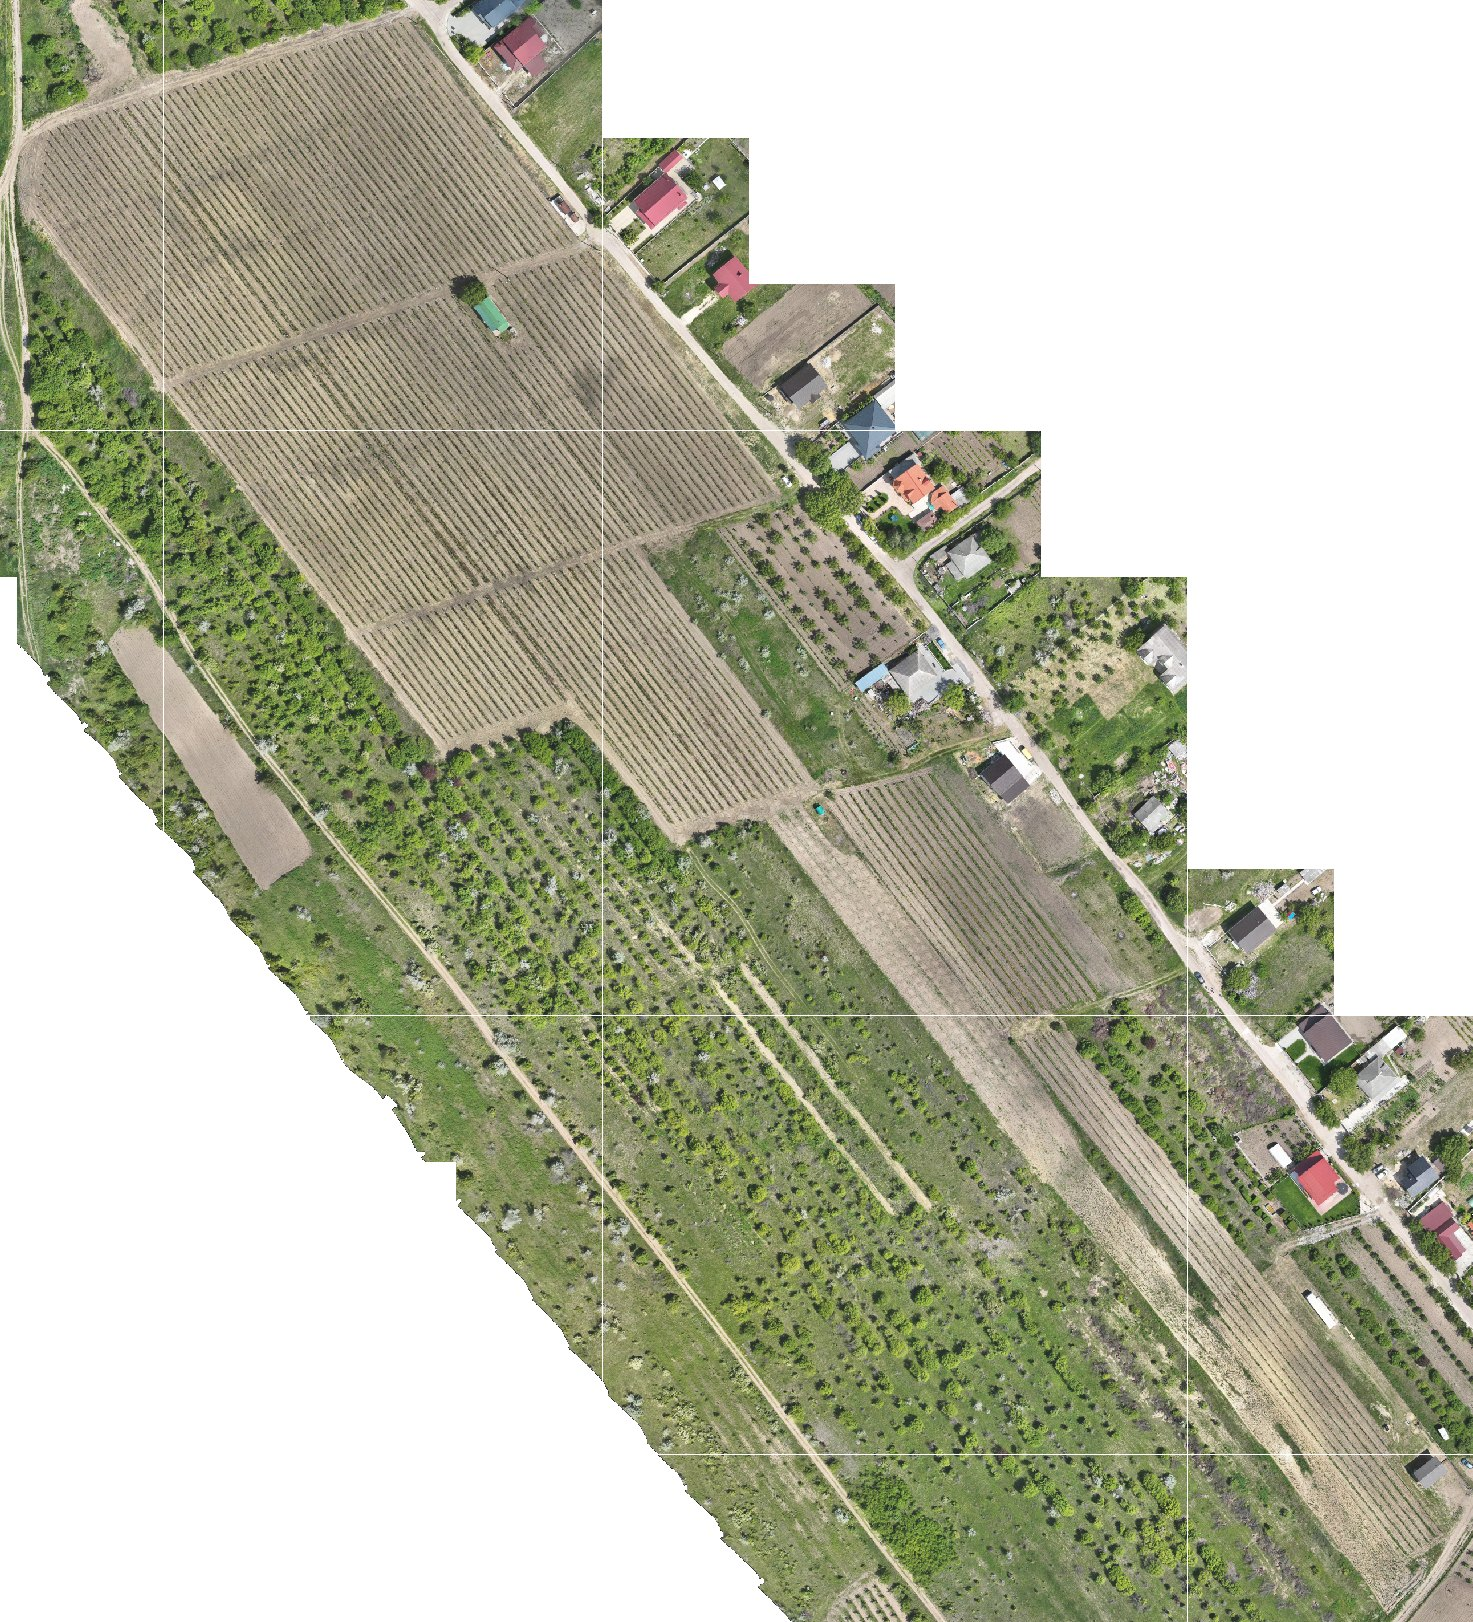
\includegraphics[width=5.721cm,height=6.300cm]{farm_ortho.jpg}};
\draw[white, line width=0.6pt, dash pattern=on 2pt off 1.5pt] (0.193,5.644) -- (0.201,5.627) -- (0.203,5.605) -- (0.194,5.570) -- (0.187,5.555) -- (0.176,5.544) -- (0.158,5.534) -- (0.143,5.517) -- (0.124,5.508) -- (0.098,5.507) -- (0.070,5.519) -- (0.071,5.462) -- (0.272,5.197) -- (0.355,5.194) -- (0.380,5.185) -- (0.408,5.158) -- (0.452,5.097) -- (0.483,5.072) -- (0.504,5.027) -- (0.631,4.855) -- (0.637,4.835) -- (0.639,4.762) -- (0.732,4.637) -- (0.744,4.616) -- (1.171,4.060) -- (1.219,4.059) -- (1.234,4.055) -- (1.248,4.047) -- (1.271,4.024) -- (1.315,3.961) -- (1.389,3.863) -- (1.404,3.849) -- (1.420,3.822) -- (1.448,3.791) -- (1.461,3.769) -- (1.499,3.724) -- (1.516,3.697) -- (1.675,3.490) -- (2.026,3.490) -- (2.029,3.514) -- (2.041,3.533) -- (2.059,3.546) -- (2.081,3.551) -- (2.121,3.548) -- (2.137,3.542) -- (2.150,3.532) -- (2.183,3.490) -- (2.216,3.490) -- (2.231,3.511) -- (2.255,3.523) -- (2.271,3.525) -- (2.291,3.520) -- (2.305,3.511) -- (2.336,3.477) -- (2.354,3.445) -- (2.616,3.098) -- (2.625,3.093) -- (2.661,3.114) -- (2.680,3.118) -- (2.695,3.131) -- (2.709,3.138) -- (2.731,3.139) -- (2.748,3.134) -- (2.793,3.155) -- (2.841,3.166) -- (2.876,3.182) -- (2.892,3.184) -- (2.910,3.180) -- (2.929,3.200) -- (2.943,3.207) -- (2.965,3.208) -- (3.002,3.238) -- (3.017,3.244) -- (3.039,3.246) -- (3.059,3.239) -- (3.076,3.248) -- (3.099,3.255) -- (3.127,3.255) -- (3.124,3.265) -- (3.111,3.278) -- (3.077,3.328) -- (2.958,3.486) -- (2.622,3.921) -- (2.583,3.976) -- (2.576,3.996) -- (2.577,4.013) -- (2.582,4.028) -- (2.600,4.048) -- (2.626,4.058) -- (2.709,4.059) -- (2.714,4.082) -- (2.728,4.103) -- (2.764,4.138) -- (2.790,4.152) -- (2.818,4.150) -- (2.838,4.140) -- (2.901,4.060) -- (2.910,4.059) -- (2.910,4.095) -- (2.898,4.117) -- (2.884,4.130) -- (2.847,4.181) -- (2.842,4.197) -- (2.843,4.218) -- (2.852,4.238) -- (2.868,4.252) -- (2.888,4.260) -- (2.910,4.259) -- (2.910,4.321) -- (2.914,4.337) -- (2.923,4.351) -- (2.946,4.367) -- (2.971,4.371) -- (2.998,4.393) -- (2.914,4.507) -- (2.910,4.523) -- (2.910,4.543) -- (2.918,4.566) -- (2.866,4.624) -- (2.838,4.627) -- (2.817,4.636) -- (2.777,4.681) -- (2.390,5.191) -- (2.361,5.225) -- (2.307,5.299) -- (2.288,5.319) -- (1.993,5.705) -- (1.983,5.723) -- (1.954,5.760) -- (1.915,5.765) -- (1.900,5.772) -- (1.888,5.784) -- (1.782,5.927) -- (1.775,5.946) -- (1.773,5.986) -- (1.756,6.013) -- (1.740,6.030) -- (1.599,6.216) -- (1.582,6.209) -- (1.560,6.208) -- (1.476,6.169) -- (1.448,6.153) -- (1.428,6.151) -- (1.409,6.156) -- (1.329,6.135) -- (1.311,6.135) -- (1.295,6.119) -- (1.276,6.109) -- (1.233,6.107) -- (1.206,6.119) -- (1.193,6.101) -- (1.180,6.092) -- (1.122,6.072) -- (1.095,6.071) -- (1.084,6.058) -- (1.065,6.047) -- (1.037,6.044) -- (1.008,6.036) -- (0.982,6.022) -- (0.958,6.016) -- (0.941,6.018) -- (0.924,6.009) -- (0.896,6.000) -- (0.864,5.993) -- (0.846,5.993) -- (0.819,5.973) -- (0.805,5.967) -- (0.722,5.942) -- (0.698,5.941) -- (0.657,5.918) -- (0.629,5.908) -- (0.606,5.907) -- (0.588,5.900) -- (0.568,5.899) -- (0.546,5.886) -- (0.520,5.876) -- (0.504,5.874) -- (0.488,5.853) -- (0.469,5.843) -- (0.448,5.840) -- (0.427,5.844) -- (0.408,5.839) -- (0.391,5.841) -- (0.369,5.830) -- (0.332,5.822) -- (0.329,5.801) -- (0.322,5.787) -- (0.311,5.775) -- (0.298,5.767) -- (0.277,5.763) -- (0.185,5.762) -- (0.196,5.742) -- (0.200,5.726) -- (0.193,5.697) -- (0.199,5.669) -- (0.193,5.644) -- cycle;
\draw[white, line width=0.6pt, dash pattern=on 2pt off 1.5pt] (3.214,3.225) -- (3.192,3.216) -- (3.171,3.216) -- (3.251,3.102) -- (3.269,3.082) -- (3.279,3.062) -- (3.339,2.978) -- (3.345,2.977) -- (3.346,2.997) -- (3.355,3.016) -- (3.367,3.028) -- (3.381,3.036) -- (3.397,3.039) -- (3.418,3.036) -- (3.432,3.028) -- (3.445,3.016) -- (3.459,2.989) -- (3.460,2.973) -- (3.456,2.956) -- (3.448,2.942) -- (3.431,2.928) -- (3.416,2.923) -- (3.395,2.922) -- (3.400,2.911) -- (3.470,2.825) -- (3.497,2.786) -- (3.668,2.568) -- (3.694,2.531) -- (3.799,2.400) -- (3.827,2.360) -- (3.836,2.354) -- (3.866,2.348) -- (3.888,2.330) -- (4.124,2.012) -- (4.131,1.997) -- (4.133,1.976) -- (4.128,1.960) -- (4.115,1.942) -- (4.102,1.933) -- (4.080,1.927) -- (4.064,1.929) -- (4.048,1.936) -- (4.098,1.868) -- (4.109,1.847) -- (4.113,1.830) -- (4.111,1.813) -- (4.104,1.798) -- (4.093,1.785) -- (4.125,1.739) -- (4.149,1.715) -- (4.185,1.665) -- (4.199,1.652) -- (4.174,1.684) -- (4.158,1.719) -- (4.157,1.736) -- (4.161,1.751) -- (4.177,1.773) -- (4.196,1.783) -- (4.214,1.785) -- (4.330,1.785) -- (4.351,1.778) -- (4.368,1.764) -- (4.404,1.714) -- (4.597,1.469) -- (4.614,1.435) -- (4.615,1.390) -- (4.654,1.339) -- (4.661,1.324) -- (4.663,1.308) -- (4.656,1.282) -- (4.642,1.265) -- (4.602,1.248) -- (4.586,1.246) -- (4.564,1.251) -- (4.547,1.264) -- (4.513,1.306) -- (4.497,1.320) -- (4.373,1.475) -- (4.361,1.495) -- (4.343,1.513) -- (4.332,1.533) -- (4.304,1.536) -- (4.282,1.549) -- (4.297,1.524) -- (4.330,1.488) -- (4.391,1.407) -- (4.454,1.328) -- (4.470,1.313) -- (4.510,1.260) -- (4.520,1.237) -- (4.519,1.217) -- (4.533,1.193) -- (4.589,1.120) -- (4.610,1.088) -- (4.617,1.033) -- (4.916,0.649) -- (4.949,0.649) -- (4.940,0.670) -- (4.940,0.692) -- (4.949,0.712) -- (4.969,0.730) -- (4.984,0.735) -- (5.001,0.736) -- (5.017,0.732) -- (5.035,0.719) -- (5.126,0.604) -- (5.137,0.583) -- (5.154,0.564) -- (5.178,0.529) -- (5.183,0.513) -- (5.183,0.486) -- (5.212,0.441) -- (5.217,0.421) -- (5.215,0.405) -- (5.209,0.390) -- (5.185,0.365) -- (5.295,0.225) -- (5.315,0.195) -- (5.331,0.181) -- (5.354,0.146) -- (5.408,0.082) -- (5.462,0.082) -- (5.496,0.124) -- (5.510,0.132) -- (5.527,0.137) -- (5.525,0.154) -- (5.530,0.175) -- (5.539,0.189) -- (5.555,0.203) -- (5.563,0.221) -- (5.573,0.233) -- (5.580,0.251) -- (5.607,0.293) -- (5.607,0.318) -- (5.622,0.354) -- (5.652,0.385) -- (5.479,0.602) -- (5.460,0.634) -- (5.453,0.653) -- (5.381,0.741) -- (5.192,0.987) -- (5.183,1.012) -- (5.182,1.090) -- (5.091,1.210) -- (5.084,1.217) -- (5.015,1.220) -- (5.000,1.227) -- (4.983,1.242) -- (4.632,1.706) -- (4.586,1.757) -- (4.578,1.773) -- (4.573,1.790) -- (4.200,2.268) -- (4.193,2.283) -- (4.192,2.305) -- (4.196,2.321) -- (4.205,2.335) -- (4.218,2.345) -- (4.239,2.353) -- (4.332,2.354) -- (4.326,2.379) -- (4.331,2.413) -- (4.312,2.433) -- (4.289,2.468) -- (4.270,2.487) -- (4.196,2.589) -- (4.145,2.651) -- (4.136,2.667) -- (4.113,2.692) -- (4.090,2.728) -- (4.078,2.739) -- (4.055,2.769) -- (4.047,2.793) -- (4.046,2.893) -- (4.033,2.915) -- (4.022,2.921) -- (3.951,2.923) -- (3.935,2.929) -- (3.918,2.944) -- (3.896,2.975) -- (3.891,3.001) -- (3.898,3.027) -- (3.924,3.052) -- (3.923,3.057) -- (3.904,3.078) -- (3.869,3.130) -- (3.596,3.489) -- (3.480,3.490) -- (3.460,3.480) -- (3.444,3.478) -- (3.428,3.480) -- (3.409,3.489) -- (3.387,3.489) -- (3.399,3.466) -- (3.468,3.371) -- (3.500,3.319) -- (3.503,3.303) -- (3.501,3.287) -- (3.495,3.272) -- (3.481,3.256) -- (3.467,3.248) -- (3.443,3.244) -- (3.430,3.231) -- (3.411,3.221) -- (3.390,3.220) -- (3.369,3.225) -- (3.352,3.199) -- (3.339,3.190) -- (3.324,3.185) -- (3.302,3.186) -- (3.275,3.199) -- (3.246,3.203) -- (3.214,3.225) -- cycle;
\draw[white, line width=0.6pt, dash pattern=on 2pt off 1.5pt] (4.199,1.652) -- (4.213,1.629) -- (4.225,1.620) -- (4.219,1.633) -- (4.199,1.652) -- cycle;
\draw[white, line width=0.6pt, dash pattern=on 2pt off 1.5pt] (0.085,5.631) -- (0.078,5.645) -- (0.070,5.653) -- (0.070,5.645) -- (0.085,5.631) -- cycle;
\draw[white, opacity=0.85, line width=1.5pt] (3.896,2.625) -- (3.893,2.622) -- (4.102,2.349) -- (4.118,2.334) -- (4.126,2.372) -- (4.159,2.341) -- (4.542,1.852) -- (4.196,2.295) -- (4.241,2.330) -- (4.282,2.330) -- (4.354,2.350) -- (3.823,3.043) -- (3.481,3.498) -- (3.508,3.513) -- (3.972,2.901) -- (4.001,2.925) -- (4.023,2.897) -- (4.001,2.925) -- (3.972,2.901) -- (3.891,3.006) -- (3.947,3.049) -- (3.595,3.513) -- (3.508,3.513) -- (3.461,3.462) -- (3.583,3.303) -- (3.466,3.458) -- (3.449,3.473) -- (3.403,3.495) -- (3.410,3.473) -- (3.548,3.292) -- (3.410,3.473) -- (3.403,3.495) -- (3.389,3.513) -- (3.364,3.493) -- (3.497,3.306) -- (3.445,3.266) -- (3.371,3.249) -- (3.346,3.230) -- (3.278,3.223) -- (3.218,3.249) -- (3.148,3.251) -- (3.016,3.429) -- (2.583,3.994) -- (2.631,4.032) -- (2.598,4.089) -- (1.780,5.162) -- (1.763,5.179) -- (1.741,5.171) -- (1.774,5.109) -- (2.138,4.637) -- (2.148,4.617) -- (2.466,4.199) -- (2.364,4.333) -- (2.340,4.315) -- (1.692,5.155) -- (1.538,5.104) -- (1.281,5.440) -- (1.538,5.104) -- (1.443,5.072) -- (1.356,5.187) -- (1.736,4.689) -- (1.443,5.072) -- (1.415,5.063) -- (1.409,5.069) -- (0.734,5.957) -- (0.698,5.962) -- (0.647,5.924) -- (0.675,5.886) -- (0.639,5.934) -- (0.569,5.922) -- (0.516,5.885) -- (0.737,5.595) -- (0.514,5.888) -- (0.489,5.860) -- (0.721,5.559) -- (0.489,5.860) -- (0.514,5.888) -- (0.537,5.906) -- (0.568,5.869) -- (0.551,5.888) -- (0.605,5.927) -- (0.668,5.946) -- (1.252,5.170) -- (2.228,3.899) -- (2.104,4.061) -- (2.129,4.081) -- (2.192,4.099) -- (2.894,3.175) -- (2.826,3.160) -- (2.688,3.343) -- (2.826,3.162) -- (2.826,3.160) -- (2.763,3.142) -- (2.726,3.191) -- (2.763,3.142) -- (2.738,3.124) -- (2.037,4.047) -- (1.987,4.008) -- (2.201,3.726) -- (1.973,4.026) -- (1.917,4.009) -- (1.983,3.922) -- (1.513,4.532) -- (1.512,4.559) -- (1.434,4.667) -- (1.425,4.688) -- (1.196,4.990) -- (1.157,4.977) -- (1.006,5.179) -- (1.157,4.977) -- (1.052,4.942) -- (0.892,5.151) -- (1.052,4.942) -- (0.992,4.922) -- (0.336,5.792) -- (0.287,5.753) -- (0.625,5.303) -- (0.275,5.768) -- (0.301,5.786) -- (0.333,5.846) -- (0.877,5.122) -- (1.764,3.961) -- (1.671,3.931) -- (2.011,3.485) -- (1.890,3.485) -- (1.798,3.607) -- (1.890,3.485) -- (1.735,3.485) -- (1.407,3.917) -- (1.735,3.485) -- (1.700,3.485) -- (1.418,3.855) -- (1.700,3.485) -- (1.851,3.485) -- (1.266,4.253) -- (1.543,3.891) -- (1.512,3.881) -- (1.537,3.849) -- (0.774,4.850) -- (0.836,4.871) -- (1.128,4.485) -- (0.836,4.871) -- (0.805,4.860) -- (0.195,5.669) -- (0.174,5.589) -- (0.150,5.571) -- (0.144,5.579) -- (0.150,5.571) -- (0.174,5.589) -- (0.742,4.839) -- (0.680,4.818) -- (0.839,4.611) -- (0.636,4.877) -- (0.451,5.127) -- (0.382,5.214) -- (0.178,5.484) -- (0.170,5.492) -- (0.131,5.463) -- (0.085,5.524) -- (0.067,5.541) -- (0.067,5.741) -- (0.184,5.791) -- (0.212,5.749) -- (0.868,4.881) -- (0.900,4.892) -- (1.638,3.921) -- (1.671,3.931) -- (1.263,4.468) -- (0.930,4.902) -- (0.992,4.922) -- (1.733,3.951) -- (1.824,3.979) -- (2.214,3.467) -- (2.278,3.516) -- (2.238,3.569) -- (1.903,4.004) -- (1.824,3.979) -- (1.080,4.952) -- (1.157,4.977) -- (1.186,4.939) -- (1.195,4.918) -- (1.359,4.701) -- (1.195,4.918) -- (1.186,4.939) -- (1.157,4.977) -- (1.257,5.011) -- (1.721,4.403) -- (1.992,4.053) -- (2.024,4.065) -- (0.887,5.552) -- (1.291,5.022) -- (1.474,5.083) -- (1.765,4.702) -- (1.474,5.083) -- (1.507,5.093) -- (1.099,5.627) -- (2.252,4.119) -- (2.315,4.140) -- (1.569,5.114) -- (1.600,5.124) -- (1.339,5.467) -- (1.600,5.124) -- (1.725,5.166) -- (1.057,6.039) -- (1.097,6.094) -- (1.160,6.108) -- (1.252,5.983) -- (1.804,5.265) -- (1.894,5.139) -- (2.595,4.228) -- (2.601,4.225) -- (2.654,4.259) -- (1.925,5.209) -- (1.917,5.220) -- (1.916,5.229) -- (1.943,5.237) -- (1.264,6.121) -- (1.313,6.158) -- (1.364,6.090) -- (1.326,6.140) -- (1.378,6.172) -- (2.071,5.273) -- (2.038,5.264) -- (2.761,4.320) -- (2.911,4.341) -- (2.931,4.403) -- (2.229,5.318) -- (2.261,5.327) -- (2.266,5.321) -- (1.562,6.231) -- (1.517,6.196) -- (1.533,6.170) -- (2.198,5.309) -- (2.166,5.300) -- (2.903,4.340) -- (2.869,4.335) -- (1.454,6.174) -- (1.378,6.172) -- (1.347,6.163) -- (1.298,6.126) -- (2.705,4.293) -- (2.731,4.309) -- (2.868,4.129) -- (2.731,4.309) -- (2.626,4.241) -- (2.653,4.205) -- (2.626,4.241) -- (2.576,4.209) -- (1.223,5.971) -- (1.130,6.096) -- (1.039,6.068) -- (0.989,6.030) -- (1.176,5.777) -- (1.284,5.645) -- (1.214,5.731) -- (1.190,5.713) -- (2.379,4.161) -- (2.347,4.150) -- (2.038,4.553) -- (2.347,4.150) -- (2.315,4.140) -- (2.761,3.559) -- (2.999,3.241) -- (3.011,3.222) -- (2.963,3.185) -- (2.895,3.272) -- (2.963,3.185) -- (3.038,3.242) -- (3.049,3.227) -- (3.074,3.246) -- (2.862,3.530) -- (2.898,3.480) -- (2.924,3.498) -- (3.110,3.250) -- (3.178,3.238) -- (3.206,3.205) -- (3.353,2.993) -- (3.412,2.927) -- (3.858,2.349) -- (4.031,2.113) -- (4.262,1.815) -- (4.274,1.807) -- (4.293,1.782) -- (4.308,1.769) -- (4.331,1.785) -- (4.353,1.759) -- (3.455,2.922) -- (3.482,2.944) -- (3.489,2.937) -- (3.987,2.290) -- (3.360,3.101) -- (3.327,3.149) -- (3.307,3.182) -- (3.380,3.237) -- (3.494,3.093) -- (4.123,2.266) -- (5.391,0.646) -- (5.402,0.626) -- (5.592,0.382) -- (5.637,0.333) -- (5.628,0.287) -- (5.581,0.235) -- (5.554,0.197) -- (5.529,0.217) -- (5.523,0.213) -- (5.490,0.255) -- (5.523,0.213) -- (5.502,0.196) -- (5.404,0.316) -- (5.534,0.155) -- (5.496,0.108) -- (5.043,0.688) -- (5.034,0.694) -- (5.029,0.706) -- (4.913,0.856) -- (4.878,0.829) -- (4.334,1.504) -- (4.315,1.533) -- (4.095,1.808) -- (4.087,1.802) -- (4.092,1.778) -- (4.517,1.237) -- (4.523,1.221) -- (4.528,1.223) -- (4.539,1.203) -- (4.610,1.118) -- (4.840,0.822) -- (4.973,0.646) -- (5.024,0.679) -- (5.171,0.489) -- (5.217,0.416) -- (5.248,0.382) -- (5.315,0.296) -- (5.321,0.283) -- (5.420,0.156) -- (5.473,0.080) -- (5.463,0.067) -- (5.415,0.106) -- (5.354,0.184) -- (5.415,0.106) -- (5.463,0.067) -- (5.615,0.254) -- (5.606,0.309) -- (5.609,0.311) -- (5.598,0.326) -- (5.646,0.359) -- (5.443,0.620) -- (5.446,0.622) -- (5.422,0.660) -- (5.067,1.112) -- (4.980,1.218) -- (4.605,1.705) -- (4.549,1.773) -- (4.539,1.794) -- (4.118,2.334) -- (4.102,2.349) -- (3.893,2.622) -- (3.896,2.625);
\draw[sxViolet, line width=0.8pt] (3.896,2.625) -- (3.893,2.622) -- (4.102,2.349) -- (4.118,2.334) -- (4.126,2.372) -- (4.159,2.341) -- (4.542,1.852) -- (4.196,2.295) -- (4.241,2.330) -- (4.282,2.330) -- (4.354,2.350) -- (3.823,3.043) -- (3.481,3.498) -- (3.508,3.513) -- (3.972,2.901) -- (4.001,2.925) -- (4.023,2.897) -- (4.001,2.925) -- (3.972,2.901) -- (3.891,3.006) -- (3.947,3.049) -- (3.595,3.513) -- (3.508,3.513) -- (3.461,3.462) -- (3.583,3.303) -- (3.466,3.458) -- (3.449,3.473) -- (3.403,3.495) -- (3.410,3.473) -- (3.548,3.292) -- (3.410,3.473) -- (3.403,3.495) -- (3.389,3.513) -- (3.364,3.493) -- (3.497,3.306) -- (3.445,3.266) -- (3.371,3.249) -- (3.346,3.230) -- (3.278,3.223) -- (3.218,3.249) -- (3.148,3.251) -- (3.016,3.429) -- (2.583,3.994) -- (2.631,4.032) -- (2.598,4.089) -- (1.780,5.162) -- (1.763,5.179) -- (1.741,5.171) -- (1.774,5.109) -- (2.138,4.637) -- (2.148,4.617) -- (2.466,4.199) -- (2.364,4.333) -- (2.340,4.315) -- (1.692,5.155) -- (1.538,5.104) -- (1.281,5.440) -- (1.538,5.104) -- (1.443,5.072) -- (1.356,5.187) -- (1.736,4.689) -- (1.443,5.072) -- (1.415,5.063) -- (1.409,5.069) -- (0.734,5.957) -- (0.698,5.962) -- (0.647,5.924) -- (0.675,5.886) -- (0.639,5.934) -- (0.569,5.922) -- (0.516,5.885) -- (0.737,5.595) -- (0.514,5.888) -- (0.489,5.860) -- (0.721,5.559) -- (0.489,5.860) -- (0.514,5.888) -- (0.537,5.906) -- (0.568,5.869) -- (0.551,5.888) -- (0.605,5.927) -- (0.668,5.946) -- (1.252,5.170) -- (2.228,3.899) -- (2.104,4.061) -- (2.129,4.081) -- (2.192,4.099) -- (2.894,3.175) -- (2.826,3.160) -- (2.688,3.343) -- (2.826,3.162) -- (2.826,3.160) -- (2.763,3.142) -- (2.726,3.191) -- (2.763,3.142) -- (2.738,3.124) -- (2.037,4.047) -- (1.987,4.008) -- (2.201,3.726) -- (1.973,4.026) -- (1.917,4.009) -- (1.983,3.922) -- (1.513,4.532) -- (1.512,4.559) -- (1.434,4.667) -- (1.425,4.688) -- (1.196,4.990) -- (1.157,4.977) -- (1.006,5.179) -- (1.157,4.977) -- (1.052,4.942) -- (0.892,5.151) -- (1.052,4.942) -- (0.992,4.922) -- (0.336,5.792) -- (0.287,5.753) -- (0.625,5.303) -- (0.275,5.768) -- (0.301,5.786) -- (0.333,5.846) -- (0.877,5.122) -- (1.764,3.961) -- (1.671,3.931) -- (2.011,3.485) -- (1.890,3.485) -- (1.798,3.607) -- (1.890,3.485) -- (1.735,3.485) -- (1.407,3.917) -- (1.735,3.485) -- (1.700,3.485) -- (1.418,3.855) -- (1.700,3.485) -- (1.851,3.485) -- (1.266,4.253) -- (1.543,3.891) -- (1.512,3.881) -- (1.537,3.849) -- (0.774,4.850) -- (0.836,4.871) -- (1.128,4.485) -- (0.836,4.871) -- (0.805,4.860) -- (0.195,5.669) -- (0.174,5.589) -- (0.150,5.571) -- (0.144,5.579) -- (0.150,5.571) -- (0.174,5.589) -- (0.742,4.839) -- (0.680,4.818) -- (0.839,4.611) -- (0.636,4.877) -- (0.451,5.127) -- (0.382,5.214) -- (0.178,5.484) -- (0.170,5.492) -- (0.131,5.463) -- (0.085,5.524) -- (0.067,5.541) -- (0.067,5.741) -- (0.184,5.791) -- (0.212,5.749) -- (0.868,4.881) -- (0.900,4.892) -- (1.638,3.921) -- (1.671,3.931) -- (1.263,4.468) -- (0.930,4.902) -- (0.992,4.922) -- (1.733,3.951) -- (1.824,3.979) -- (2.214,3.467) -- (2.278,3.516) -- (2.238,3.569) -- (1.903,4.004) -- (1.824,3.979) -- (1.080,4.952) -- (1.157,4.977) -- (1.186,4.939) -- (1.195,4.918) -- (1.359,4.701) -- (1.195,4.918) -- (1.186,4.939) -- (1.157,4.977) -- (1.257,5.011) -- (1.721,4.403) -- (1.992,4.053) -- (2.024,4.065) -- (0.887,5.552) -- (1.291,5.022) -- (1.474,5.083) -- (1.765,4.702) -- (1.474,5.083) -- (1.507,5.093) -- (1.099,5.627) -- (2.252,4.119) -- (2.315,4.140) -- (1.569,5.114) -- (1.600,5.124) -- (1.339,5.467) -- (1.600,5.124) -- (1.725,5.166) -- (1.057,6.039) -- (1.097,6.094) -- (1.160,6.108) -- (1.252,5.983) -- (1.804,5.265) -- (1.894,5.139) -- (2.595,4.228) -- (2.601,4.225) -- (2.654,4.259) -- (1.925,5.209) -- (1.917,5.220) -- (1.916,5.229) -- (1.943,5.237) -- (1.264,6.121) -- (1.313,6.158) -- (1.364,6.090) -- (1.326,6.140) -- (1.378,6.172) -- (2.071,5.273) -- (2.038,5.264) -- (2.761,4.320) -- (2.911,4.341) -- (2.931,4.403) -- (2.229,5.318) -- (2.261,5.327) -- (2.266,5.321) -- (1.562,6.231) -- (1.517,6.196) -- (1.533,6.170) -- (2.198,5.309) -- (2.166,5.300) -- (2.903,4.340) -- (2.869,4.335) -- (1.454,6.174) -- (1.378,6.172) -- (1.347,6.163) -- (1.298,6.126) -- (2.705,4.293) -- (2.731,4.309) -- (2.868,4.129) -- (2.731,4.309) -- (2.626,4.241) -- (2.653,4.205) -- (2.626,4.241) -- (2.576,4.209) -- (1.223,5.971) -- (1.130,6.096) -- (1.039,6.068) -- (0.989,6.030) -- (1.176,5.777) -- (1.284,5.645) -- (1.214,5.731) -- (1.190,5.713) -- (2.379,4.161) -- (2.347,4.150) -- (2.038,4.553) -- (2.347,4.150) -- (2.315,4.140) -- (2.761,3.559) -- (2.999,3.241) -- (3.011,3.222) -- (2.963,3.185) -- (2.895,3.272) -- (2.963,3.185) -- (3.038,3.242) -- (3.049,3.227) -- (3.074,3.246) -- (2.862,3.530) -- (2.898,3.480) -- (2.924,3.498) -- (3.110,3.250) -- (3.178,3.238) -- (3.206,3.205) -- (3.353,2.993) -- (3.412,2.927) -- (3.858,2.349) -- (4.031,2.113) -- (4.262,1.815) -- (4.274,1.807) -- (4.293,1.782) -- (4.308,1.769) -- (4.331,1.785) -- (4.353,1.759) -- (3.455,2.922) -- (3.482,2.944) -- (3.489,2.937) -- (3.987,2.290) -- (3.360,3.101) -- (3.327,3.149) -- (3.307,3.182) -- (3.380,3.237) -- (3.494,3.093) -- (4.123,2.266) -- (5.391,0.646) -- (5.402,0.626) -- (5.592,0.382) -- (5.637,0.333) -- (5.628,0.287) -- (5.581,0.235) -- (5.554,0.197) -- (5.529,0.217) -- (5.523,0.213) -- (5.490,0.255) -- (5.523,0.213) -- (5.502,0.196) -- (5.404,0.316) -- (5.534,0.155) -- (5.496,0.108) -- (5.043,0.688) -- (5.034,0.694) -- (5.029,0.706) -- (4.913,0.856) -- (4.878,0.829) -- (4.334,1.504) -- (4.315,1.533) -- (4.095,1.808) -- (4.087,1.802) -- (4.092,1.778) -- (4.517,1.237) -- (4.523,1.221) -- (4.528,1.223) -- (4.539,1.203) -- (4.610,1.118) -- (4.840,0.822) -- (4.973,0.646) -- (5.024,0.679) -- (5.171,0.489) -- (5.217,0.416) -- (5.248,0.382) -- (5.315,0.296) -- (5.321,0.283) -- (5.420,0.156) -- (5.473,0.080) -- (5.463,0.067) -- (5.415,0.106) -- (5.354,0.184) -- (5.415,0.106) -- (5.463,0.067) -- (5.615,0.254) -- (5.606,0.309) -- (5.609,0.311) -- (5.598,0.326) -- (5.646,0.359) -- (5.443,0.620) -- (5.446,0.622) -- (5.422,0.660) -- (5.067,1.112) -- (4.980,1.218) -- (4.605,1.705) -- (4.549,1.773) -- (4.539,1.794) -- (4.118,2.334) -- (4.102,2.349) -- (3.893,2.622) -- (3.896,2.625);
\filldraw[fill=sxAmber, draw=white, line width=0.2pt] (4.202,2.297) circle (0.8pt);
\filldraw[fill=sxAmber, draw=white, line width=0.2pt] (4.543,1.850) circle (0.8pt);
\filldraw[fill=sxAmber, draw=white, line width=0.2pt] (4.457,1.962) circle (0.8pt);
\filldraw[fill=sxAmber, draw=white, line width=0.2pt] (4.372,2.074) circle (0.8pt);
\filldraw[fill=sxAmber, draw=white, line width=0.2pt] (4.287,2.186) circle (0.8pt);
\filldraw[fill=sxAmber, draw=white, line width=0.2pt] (4.313,2.431) circle (0.8pt);
\filldraw[fill=sxAmber, draw=white, line width=0.2pt] (4.251,2.512) circle (0.8pt);
\filldraw[fill=sxAmber, draw=white, line width=0.2pt] (4.158,2.633) circle (0.8pt);
\filldraw[fill=sxAmber, draw=white, line width=0.2pt] (4.114,2.691) circle (0.8pt);
\filldraw[fill=sxAmber, draw=white, line width=0.2pt] (4.006,2.831) circle (0.8pt);
\filldraw[fill=sxAmber, draw=white, line width=0.2pt] (3.913,2.950) circle (0.8pt);
\filldraw[fill=sxAmber, draw=white, line width=0.2pt] (3.836,3.052) circle (0.8pt);
\filldraw[fill=sxAmber, draw=white, line width=0.2pt] (3.607,3.304) circle (0.8pt);
\filldraw[fill=sxAmber, draw=white, line width=0.2pt] (3.545,3.437) circle (0.8pt);
\filldraw[fill=sxAmber, draw=white, line width=0.2pt] (3.509,3.434) circle (0.8pt);
\filldraw[fill=sxAmber, draw=white, line width=0.2pt] (3.645,3.326) circle (0.8pt);
\filldraw[fill=sxAmber, draw=white, line width=0.2pt] (4.008,2.886) circle (0.8pt);
\filldraw[fill=sxAmber, draw=white, line width=0.2pt] (3.895,3.090) circle (0.8pt);
\filldraw[fill=sxAmber, draw=white, line width=0.2pt] (3.852,3.147) circle (0.8pt);
\filldraw[fill=sxAmber, draw=white, line width=0.2pt] (3.841,3.388) circle (0.8pt);
\filldraw[fill=sxAmber, draw=white, line width=0.2pt] (3.575,3.559) circle (0.8pt);
\filldraw[fill=sxAmber, draw=white, line width=0.2pt] (3.568,3.291) circle (0.8pt);
\filldraw[fill=sxAmber, draw=white, line width=0.2pt] (3.521,3.352) circle (0.8pt);
\filldraw[fill=sxAmber, draw=white, line width=0.2pt] (3.489,3.394) circle (0.8pt);
\filldraw[fill=sxAmber, draw=white, line width=0.2pt] (3.536,3.282) circle (0.8pt);
\filldraw[fill=sxAmber, draw=white, line width=0.2pt] (3.430,3.426) circle (0.8pt);
\filldraw[fill=sxAmber, draw=white, line width=0.2pt] (2.994,3.432) circle (0.8pt);
\filldraw[fill=sxAmber, draw=white, line width=0.2pt] (2.531,4.199) circle (0.8pt);
\filldraw[fill=sxAmber, draw=white, line width=0.2pt] (2.196,4.636) circle (0.8pt);
\filldraw[fill=sxAmber, draw=white, line width=0.2pt] (1.952,4.960) circle (0.8pt);
\filldraw[fill=sxAmber, draw=white, line width=0.2pt] (1.776,5.072) circle (0.8pt);
\filldraw[fill=sxAmber, draw=white, line width=0.2pt] (1.831,5.069) circle (0.8pt);
\filldraw[fill=sxAmber, draw=white, line width=0.2pt] (1.911,4.897) circle (0.8pt);
\filldraw[fill=sxAmber, draw=white, line width=0.2pt] (1.983,4.871) circle (0.8pt);
\filldraw[fill=sxAmber, draw=white, line width=0.2pt] (1.987,4.800) circle (0.8pt);
\filldraw[fill=sxAmber, draw=white, line width=0.2pt] (2.024,4.818) circle (0.8pt);
\filldraw[fill=sxAmber, draw=white, line width=0.2pt] (2.010,4.770) circle (0.8pt);
\filldraw[fill=sxAmber, draw=white, line width=0.2pt] (2.134,4.673) circle (0.8pt);
\filldraw[fill=sxAmber, draw=white, line width=0.2pt] (2.147,4.593) circle (0.8pt);
\filldraw[fill=sxAmber, draw=white, line width=0.2pt] (2.207,4.514) circle (0.8pt);
\filldraw[fill=sxAmber, draw=white, line width=0.2pt] (2.233,4.530) circle (0.8pt);
\filldraw[fill=sxAmber, draw=white, line width=0.2pt] (2.230,4.485) circle (0.8pt);
\filldraw[fill=sxAmber, draw=white, line width=0.2pt] (2.478,4.208) circle (0.8pt);
\filldraw[fill=sxAmber, draw=white, line width=0.2pt] (2.157,4.529) circle (0.8pt);
\filldraw[fill=sxAmber, draw=white, line width=0.2pt] (2.072,4.640) circle (0.8pt);
\filldraw[fill=sxAmber, draw=white, line width=0.2pt] (1.295,5.450) circle (0.8pt);
\filldraw[fill=sxAmber, draw=white, line width=0.2pt] (1.368,5.196) circle (0.8pt);
\filldraw[fill=sxAmber, draw=white, line width=0.2pt] (1.724,4.680) circle (0.8pt);
\filldraw[fill=sxAmber, draw=white, line width=0.2pt] (1.275,5.220) circle (0.8pt);
\filldraw[fill=sxAmber, draw=white, line width=0.2pt] (1.088,5.465) circle (0.8pt);
\filldraw[fill=sxAmber, draw=white, line width=0.2pt] (1.083,5.520) circle (0.8pt);
\filldraw[fill=sxAmber, draw=white, line width=0.2pt] (0.882,5.735) circle (0.8pt);
\filldraw[fill=sxAmber, draw=white, line width=0.2pt] (0.663,5.877) circle (0.8pt);
\filldraw[fill=sxAmber, draw=white, line width=0.2pt] (0.725,5.586) circle (0.8pt);
\filldraw[fill=sxAmber, draw=white, line width=0.2pt] (0.547,5.819) circle (0.8pt);
\filldraw[fill=sxAmber, draw=white, line width=0.2pt] (0.705,5.547) circle (0.8pt);
\filldraw[fill=sxAmber, draw=white, line width=0.2pt] (0.554,5.858) circle (0.8pt);
\filldraw[fill=sxAmber, draw=white, line width=0.2pt] (0.905,5.655) circle (0.8pt);
\filldraw[fill=sxAmber, draw=white, line width=0.2pt] (1.081,5.370) circle (0.8pt);
\filldraw[fill=sxAmber, draw=white, line width=0.2pt] (1.257,5.190) circle (0.8pt);
\filldraw[fill=sxAmber, draw=white, line width=0.2pt] (1.453,4.934) circle (0.8pt);
\filldraw[fill=sxAmber, draw=white, line width=0.2pt] (1.541,4.819) circle (0.8pt);
\filldraw[fill=sxAmber, draw=white, line width=0.2pt] (1.729,4.526) circle (0.8pt);
\filldraw[fill=sxAmber, draw=white, line width=0.2pt] (1.880,4.327) circle (0.8pt);
\filldraw[fill=sxAmber, draw=white, line width=0.2pt] (1.911,4.334) circle (0.8pt);
\filldraw[fill=sxAmber, draw=white, line width=0.2pt] (2.080,4.067) circle (0.8pt);
\filldraw[fill=sxAmber, draw=white, line width=0.2pt] (2.240,3.909) circle (0.8pt);
\filldraw[fill=sxAmber, draw=white, line width=0.2pt] (2.211,3.946) circle (0.8pt);
\filldraw[fill=sxAmber, draw=white, line width=0.2pt] (2.299,3.982) circle (0.8pt);
\filldraw[fill=sxAmber, draw=white, line width=0.2pt] (2.483,3.695) circle (0.8pt);
\filldraw[fill=sxAmber, draw=white, line width=0.2pt] (2.616,3.520) circle (0.8pt);
\filldraw[fill=sxAmber, draw=white, line width=0.2pt] (2.856,3.198) circle (0.8pt);
\filldraw[fill=sxAmber, draw=white, line width=0.2pt] (2.699,3.352) circle (0.8pt);
\filldraw[fill=sxAmber, draw=white, line width=0.2pt] (2.738,3.200) circle (0.8pt);
\filldraw[fill=sxAmber, draw=white, line width=0.2pt] (2.658,3.255) circle (0.8pt);
\filldraw[fill=sxAmber, draw=white, line width=0.2pt] (2.495,3.419) circle (0.8pt);
\filldraw[fill=sxAmber, draw=white, line width=0.2pt] (2.466,3.457) circle (0.8pt);
\filldraw[fill=sxAmber, draw=white, line width=0.2pt] (2.050,4.056) circle (0.8pt);
\filldraw[fill=sxAmber, draw=white, line width=0.2pt] (2.188,3.716) circle (0.8pt);
\filldraw[fill=sxAmber, draw=white, line width=0.2pt] (1.972,3.915) circle (0.8pt);
\filldraw[fill=sxAmber, draw=white, line width=0.2pt] (1.875,4.044) circle (0.8pt);
\filldraw[fill=sxAmber, draw=white, line width=0.2pt] (1.777,4.173) circle (0.8pt);
\filldraw[fill=sxAmber, draw=white, line width=0.2pt] (1.679,4.303) circle (0.8pt);
\filldraw[fill=sxAmber, draw=white, line width=0.2pt] (1.582,4.432) circle (0.8pt);
\filldraw[fill=sxAmber, draw=white, line width=0.2pt] (1.484,4.561) circle (0.8pt);
\filldraw[fill=sxAmber, draw=white, line width=0.2pt] (1.356,4.799) circle (0.8pt);
\filldraw[fill=sxAmber, draw=white, line width=0.2pt] (1.316,4.853) circle (0.8pt);
\filldraw[fill=sxAmber, draw=white, line width=0.2pt] (1.245,4.947) circle (0.8pt);
\filldraw[fill=sxAmber, draw=white, line width=0.2pt] (0.990,5.167) circle (0.8pt);
\filldraw[fill=sxAmber, draw=white, line width=0.2pt] (1.090,5.101) circle (0.8pt);
\filldraw[fill=sxAmber, draw=white, line width=0.2pt] (1.125,5.055) circle (0.8pt);
\filldraw[fill=sxAmber, draw=white, line width=0.2pt] (0.903,5.159) circle (0.8pt);
\filldraw[fill=sxAmber, draw=white, line width=0.2pt] (0.897,5.070) circle (0.8pt);
\filldraw[fill=sxAmber, draw=white, line width=0.2pt] (0.814,5.131) circle (0.8pt);
\filldraw[fill=sxAmber, draw=white, line width=0.2pt] (0.640,5.361) circle (0.8pt);
\filldraw[fill=sxAmber, draw=white, line width=0.2pt] (0.606,5.458) circle (0.8pt);
\filldraw[fill=sxAmber, draw=white, line width=0.2pt] (0.514,5.581) circle (0.8pt);
\filldraw[fill=sxAmber, draw=white, line width=0.2pt] (0.325,5.729) circle (0.8pt);
\filldraw[fill=sxAmber, draw=white, line width=0.2pt] (0.365,5.675) circle (0.8pt);
\filldraw[fill=sxAmber, draw=white, line width=0.2pt] (0.453,5.558) circle (0.8pt);
\filldraw[fill=sxAmber, draw=white, line width=0.2pt] (0.514,5.423) circle (0.8pt);
\filldraw[fill=sxAmber, draw=white, line width=0.2pt] (0.637,5.313) circle (0.8pt);
\filldraw[fill=sxAmber, draw=white, line width=0.2pt] (0.512,5.480) circle (0.8pt);
\filldraw[fill=sxAmber, draw=white, line width=0.2pt] (0.331,5.666) circle (0.8pt);
\filldraw[fill=sxAmber, draw=white, line width=0.2pt] (0.446,5.715) circle (0.8pt);
\filldraw[fill=sxAmber, draw=white, line width=0.2pt] (0.512,5.629) circle (0.8pt);
\filldraw[fill=sxAmber, draw=white, line width=0.2pt] (0.609,5.501) circle (0.8pt);
\filldraw[fill=sxAmber, draw=white, line width=0.2pt] (0.689,5.395) circle (0.8pt);
\filldraw[fill=sxAmber, draw=white, line width=0.2pt] (0.806,5.241) circle (0.8pt);
\filldraw[fill=sxAmber, draw=white, line width=0.2pt] (0.839,5.197) circle (0.8pt);
\filldraw[fill=sxAmber, draw=white, line width=0.2pt] (1.353,4.522) circle (0.8pt);
\filldraw[fill=sxAmber, draw=white, line width=0.2pt] (1.378,4.489) circle (0.8pt);
\filldraw[fill=sxAmber, draw=white, line width=0.2pt] (1.573,4.183) circle (0.8pt);
\filldraw[fill=sxAmber, draw=white, line width=0.2pt] (1.605,4.141) circle (0.8pt);
\filldraw[fill=sxAmber, draw=white, line width=0.2pt] (1.697,4.022) circle (0.8pt);
\filldraw[fill=sxAmber, draw=white, line width=0.2pt] (1.706,3.858) circle (0.8pt);
\filldraw[fill=sxAmber, draw=white, line width=0.2pt] (1.884,3.675) circle (0.8pt);
\filldraw[fill=sxAmber, draw=white, line width=0.2pt] (1.810,3.616) circle (0.8pt);
\filldraw[fill=sxAmber, draw=white, line width=0.2pt] (1.568,3.683) circle (0.8pt);
\filldraw[fill=sxAmber, draw=white, line width=0.2pt] (1.419,3.926) circle (0.8pt);
\filldraw[fill=sxAmber, draw=white, line width=0.2pt] (1.436,3.855) circle (0.8pt);
\filldraw[fill=sxAmber, draw=white, line width=0.2pt] (1.471,3.857) circle (0.8pt);
\filldraw[fill=sxAmber, draw=white, line width=0.2pt] (1.530,3.733) circle (0.8pt);
\filldraw[fill=sxAmber, draw=white, line width=0.2pt] (1.448,3.791) circle (0.8pt);
\filldraw[fill=sxAmber, draw=white, line width=0.2pt] (1.407,3.845) circle (0.8pt);
\filldraw[fill=sxAmber, draw=white, line width=0.2pt] (1.502,3.720) circle (0.8pt);
\filldraw[fill=sxAmber, draw=white, line width=0.2pt] (1.755,3.639) circle (0.8pt);
\filldraw[fill=sxAmber, draw=white, line width=0.2pt] (1.660,3.713) circle (0.8pt);
\filldraw[fill=sxAmber, draw=white, line width=0.2pt] (1.519,3.947) circle (0.8pt);
\filldraw[fill=sxAmber, draw=white, line width=0.2pt] (1.356,4.159) circle (0.8pt);
\filldraw[fill=sxAmber, draw=white, line width=0.2pt] (1.278,4.262) circle (0.8pt);
\filldraw[fill=sxAmber, draw=white, line width=0.2pt] (1.499,3.873) circle (0.8pt);
\filldraw[fill=sxAmber, draw=white, line width=0.2pt] (1.524,3.839) circle (0.8pt);
\filldraw[fill=sxAmber, draw=white, line width=0.2pt] (1.325,4.101) circle (0.8pt);
\filldraw[fill=sxAmber, draw=white, line width=0.2pt] (1.264,4.180) circle (0.8pt);
\filldraw[fill=sxAmber, draw=white, line width=0.2pt] (1.148,4.332) circle (0.8pt);
\filldraw[fill=sxAmber, draw=white, line width=0.2pt] (1.140,4.494) circle (0.8pt);
\filldraw[fill=sxAmber, draw=white, line width=0.2pt] (1.106,4.488) circle (0.8pt);
\filldraw[fill=sxAmber, draw=white, line width=0.2pt] (0.680,5.053) circle (0.8pt);
\filldraw[fill=sxAmber, draw=white, line width=0.2pt] (0.618,5.133) circle (0.8pt);
\filldraw[fill=sxAmber, draw=white, line width=0.2pt] (0.589,5.122) circle (0.8pt);
\filldraw[fill=sxAmber, draw=white, line width=0.2pt] (0.590,5.170) circle (0.8pt);
\filldraw[fill=sxAmber, draw=white, line width=0.2pt] (0.470,5.280) circle (0.8pt);
\filldraw[fill=sxAmber, draw=white, line width=0.2pt] (0.491,5.301) circle (0.8pt);
\filldraw[fill=sxAmber, draw=white, line width=0.2pt] (0.426,5.388) circle (0.8pt);
\filldraw[fill=sxAmber, draw=white, line width=0.2pt] (0.361,5.425) circle (0.8pt);
\filldraw[fill=sxAmber, draw=white, line width=0.2pt] (0.375,5.455) circle (0.8pt);
\filldraw[fill=sxAmber, draw=white, line width=0.2pt] (0.325,5.522) circle (0.8pt);
\filldraw[fill=sxAmber, draw=white, line width=0.2pt] (0.298,5.557) circle (0.8pt);
\filldraw[fill=sxAmber, draw=white, line width=0.2pt] (0.277,5.586) circle (0.8pt);
\filldraw[fill=sxAmber, draw=white, line width=0.2pt] (0.210,5.627) circle (0.8pt);
\filldraw[fill=sxAmber, draw=white, line width=0.2pt] (0.229,5.649) circle (0.8pt);
\filldraw[fill=sxAmber, draw=white, line width=0.2pt] (0.131,5.569) circle (0.8pt);
\filldraw[fill=sxAmber, draw=white, line width=0.2pt] (0.220,5.554) circle (0.8pt);
\filldraw[fill=sxAmber, draw=white, line width=0.2pt] (0.271,5.487) circle (0.8pt);
\filldraw[fill=sxAmber, draw=white, line width=0.2pt] (0.303,5.444) circle (0.8pt);
\filldraw[fill=sxAmber, draw=white, line width=0.2pt] (0.288,5.416) circle (0.8pt);
\filldraw[fill=sxAmber, draw=white, line width=0.2pt] (0.314,5.382) circle (0.8pt);
\filldraw[fill=sxAmber, draw=white, line width=0.2pt] (0.364,5.364) circle (0.8pt);
\filldraw[fill=sxAmber, draw=white, line width=0.2pt] (0.411,5.302) circle (0.8pt);
\filldraw[fill=sxAmber, draw=white, line width=0.2pt] (0.451,5.249) circle (0.8pt);
\filldraw[fill=sxAmber, draw=white, line width=0.2pt] (0.451,5.200) circle (0.8pt);
\filldraw[fill=sxAmber, draw=white, line width=0.2pt] (0.533,5.091) circle (0.8pt);
\filldraw[fill=sxAmber, draw=white, line width=0.2pt] (0.574,5.087) circle (0.8pt);
\filldraw[fill=sxAmber, draw=white, line width=0.2pt] (0.623,5.023) circle (0.8pt);
\filldraw[fill=sxAmber, draw=white, line width=0.2pt] (0.827,4.602) circle (0.8pt);
\filldraw[fill=sxAmber, draw=white, line width=0.2pt] (0.478,5.066) circle (0.8pt);
\filldraw[fill=sxAmber, draw=white, line width=0.2pt] (0.408,5.158) circle (0.8pt);
\filldraw[fill=sxAmber, draw=white, line width=0.2pt] (0.386,5.187) circle (0.8pt);
\filldraw[fill=sxAmber, draw=white, line width=0.2pt] (0.370,5.253) circle (0.8pt);
\filldraw[fill=sxAmber, draw=white, line width=0.2pt] (0.317,5.277) circle (0.8pt);
\filldraw[fill=sxAmber, draw=white, line width=0.2pt] (0.322,5.316) circle (0.8pt);
\filldraw[fill=sxAmber, draw=white, line width=0.2pt] (0.282,5.322) circle (0.8pt);
\filldraw[fill=sxAmber, draw=white, line width=0.2pt] (0.258,5.401) circle (0.8pt);
\filldraw[fill=sxAmber, draw=white, line width=0.2pt] (0.219,5.406) circle (0.8pt);
\filldraw[fill=sxAmber, draw=white, line width=0.2pt] (0.213,5.461) circle (0.8pt);
\filldraw[fill=sxAmber, draw=white, line width=0.2pt] (0.106,5.470) circle (0.8pt);
\filldraw[fill=sxAmber, draw=white, line width=0.2pt] (0.250,5.722) circle (0.8pt);
\filldraw[fill=sxAmber, draw=white, line width=0.2pt] (0.284,5.678) circle (0.8pt);
\filldraw[fill=sxAmber, draw=white, line width=0.2pt] (0.331,5.616) circle (0.8pt);
\filldraw[fill=sxAmber, draw=white, line width=0.2pt] (0.372,5.562) circle (0.8pt);
\filldraw[fill=sxAmber, draw=white, line width=0.2pt] (0.406,5.517) circle (0.8pt);
\filldraw[fill=sxAmber, draw=white, line width=0.2pt] (0.438,5.475) circle (0.8pt);
\filldraw[fill=sxAmber, draw=white, line width=0.2pt] (0.417,5.455) circle (0.8pt);
\filldraw[fill=sxAmber, draw=white, line width=0.2pt] (0.469,5.434) circle (0.8pt);
\filldraw[fill=sxAmber, draw=white, line width=0.2pt] (0.528,5.356) circle (0.8pt);
\filldraw[fill=sxAmber, draw=white, line width=0.2pt] (0.537,5.296) circle (0.8pt);
\filldraw[fill=sxAmber, draw=white, line width=0.2pt] (0.573,5.297) circle (0.8pt);
\filldraw[fill=sxAmber, draw=white, line width=0.2pt] (0.615,5.242) circle (0.8pt);
\filldraw[fill=sxAmber, draw=white, line width=0.2pt] (0.980,4.760) circle (0.8pt);
\filldraw[fill=sxAmber, draw=white, line width=0.2pt] (1.064,4.650) circle (0.8pt);
\filldraw[fill=sxAmber, draw=white, line width=0.2pt] (1.252,4.458) circle (0.8pt);
\filldraw[fill=sxAmber, draw=white, line width=0.2pt] (1.266,4.385) circle (0.8pt);
\filldraw[fill=sxAmber, draw=white, line width=0.2pt] (1.509,4.064) circle (0.8pt);
\filldraw[fill=sxAmber, draw=white, line width=0.2pt] (1.546,4.070) circle (0.8pt);
\filldraw[fill=sxAmber, draw=white, line width=0.2pt] (1.572,3.980) circle (0.8pt);
\filldraw[fill=sxAmber, draw=white, line width=0.2pt] (1.354,4.374) circle (0.8pt);
\filldraw[fill=sxAmber, draw=white, line width=0.2pt] (0.971,4.823) circle (0.8pt);
\filldraw[fill=sxAmber, draw=white, line width=0.2pt] (1.339,4.442) circle (0.8pt);
\filldraw[fill=sxAmber, draw=white, line width=0.2pt] (1.963,3.820) circle (0.8pt);
\filldraw[fill=sxAmber, draw=white, line width=0.2pt] (2.159,3.520) circle (0.8pt);
\filldraw[fill=sxAmber, draw=white, line width=0.2pt] (2.185,3.531) circle (0.8pt);
\filldraw[fill=sxAmber, draw=white, line width=0.2pt] (2.168,3.656) circle (0.8pt);
\filldraw[fill=sxAmber, draw=white, line width=0.2pt] (2.142,3.657) circle (0.8pt);
\filldraw[fill=sxAmber, draw=white, line width=0.2pt] (2.070,3.785) circle (0.8pt);
\filldraw[fill=sxAmber, draw=white, line width=0.2pt] (1.998,3.844) circle (0.8pt);
\filldraw[fill=sxAmber, draw=white, line width=0.2pt] (1.791,4.045) circle (0.8pt);
\filldraw[fill=sxAmber, draw=white, line width=0.2pt] (1.740,4.066) circle (0.8pt);
\filldraw[fill=sxAmber, draw=white, line width=0.2pt] (1.590,4.307) circle (0.8pt);
\filldraw[fill=sxAmber, draw=white, line width=0.2pt] (1.540,4.326) circle (0.8pt);
\filldraw[fill=sxAmber, draw=white, line width=0.2pt] (1.458,4.479) circle (0.8pt);
\filldraw[fill=sxAmber, draw=white, line width=0.2pt] (1.422,4.479) circle (0.8pt);
\filldraw[fill=sxAmber, draw=white, line width=0.2pt] (1.386,4.526) circle (0.8pt);
\filldraw[fill=sxAmber, draw=white, line width=0.2pt] (1.346,4.692) circle (0.8pt);
\filldraw[fill=sxAmber, draw=white, line width=0.2pt] (1.286,4.946) circle (0.8pt);
\filldraw[fill=sxAmber, draw=white, line width=0.2pt] (1.330,4.942) circle (0.8pt);
\filldraw[fill=sxAmber, draw=white, line width=0.2pt] (1.489,4.678) circle (0.8pt);
\filldraw[fill=sxAmber, draw=white, line width=0.2pt] (1.680,4.431) circle (0.8pt);
\filldraw[fill=sxAmber, draw=white, line width=0.2pt] (1.736,4.461) circle (0.8pt);
\filldraw[fill=sxAmber, draw=white, line width=0.2pt] (0.874,5.542) circle (0.8pt);
\filldraw[fill=sxAmber, draw=white, line width=0.2pt] (1.056,5.354) circle (0.8pt);
\filldraw[fill=sxAmber, draw=white, line width=0.2pt] (1.755,4.691) circle (0.8pt);
\filldraw[fill=sxAmber, draw=white, line width=0.2pt] (1.486,5.146) circle (0.8pt);
\filldraw[fill=sxAmber, draw=white, line width=0.2pt] (1.342,5.284) circle (0.8pt);
\filldraw[fill=sxAmber, draw=white, line width=0.2pt] (1.293,5.348) circle (0.8pt);
\filldraw[fill=sxAmber, draw=white, line width=0.2pt] (1.169,5.512) circle (0.8pt);
\filldraw[fill=sxAmber, draw=white, line width=0.2pt] (1.088,5.619) circle (0.8pt);
\filldraw[fill=sxAmber, draw=white, line width=0.2pt] (1.319,5.315) circle (0.8pt);
\filldraw[fill=sxAmber, draw=white, line width=0.2pt] (1.580,5.024) circle (0.8pt);
\filldraw[fill=sxAmber, draw=white, line width=0.2pt] (1.622,4.916) circle (0.8pt);
\filldraw[fill=sxAmber, draw=white, line width=0.2pt] (1.672,4.904) circle (0.8pt);
\filldraw[fill=sxAmber, draw=white, line width=0.2pt] (1.647,4.882) circle (0.8pt);
\filldraw[fill=sxAmber, draw=white, line width=0.2pt] (1.721,4.840) circle (0.8pt);
\filldraw[fill=sxAmber, draw=white, line width=0.2pt] (1.701,4.811) circle (0.8pt);
\filldraw[fill=sxAmber, draw=white, line width=0.2pt] (1.770,4.777) circle (0.8pt);
\filldraw[fill=sxAmber, draw=white, line width=0.2pt] (1.778,4.712) circle (0.8pt);
\filldraw[fill=sxAmber, draw=white, line width=0.2pt] (2.055,4.404) circle (0.8pt);
\filldraw[fill=sxAmber, draw=white, line width=0.2pt] (2.058,4.347) circle (0.8pt);
\filldraw[fill=sxAmber, draw=white, line width=0.2pt] (2.104,4.339) circle (0.8pt);
\filldraw[fill=sxAmber, draw=white, line width=0.2pt] (2.118,4.268) circle (0.8pt);
\filldraw[fill=sxAmber, draw=white, line width=0.2pt] (2.193,4.169) circle (0.8pt);
\filldraw[fill=sxAmber, draw=white, line width=0.2pt] (2.227,4.177) circle (0.8pt);
\filldraw[fill=sxAmber, draw=white, line width=0.2pt] (2.050,4.513) circle (0.8pt);
\filldraw[fill=sxAmber, draw=white, line width=0.2pt] (1.997,4.528) circle (0.8pt);
\filldraw[fill=sxAmber, draw=white, line width=0.2pt] (2.017,4.556) circle (0.8pt);
\filldraw[fill=sxAmber, draw=white, line width=0.2pt] (1.897,4.658) circle (0.8pt);
\filldraw[fill=sxAmber, draw=white, line width=0.2pt] (1.793,4.848) circle (0.8pt);
\filldraw[fill=sxAmber, draw=white, line width=0.2pt] (1.751,4.850) circle (0.8pt);
\filldraw[fill=sxAmber, draw=white, line width=0.2pt] (1.681,4.942) circle (0.8pt);
\filldraw[fill=sxAmber, draw=white, line width=0.2pt] (1.325,5.456) circle (0.8pt);
\filldraw[fill=sxAmber, draw=white, line width=0.2pt] (1.418,5.334) circle (0.8pt);
\filldraw[fill=sxAmber, draw=white, line width=0.2pt] (1.465,5.273) circle (0.8pt);
\filldraw[fill=sxAmber, draw=white, line width=0.2pt] (1.641,5.251) circle (0.8pt);
\filldraw[fill=sxAmber, draw=white, line width=0.2pt] (1.566,5.401) circle (0.8pt);
\filldraw[fill=sxAmber, draw=white, line width=0.2pt] (1.322,5.667) circle (0.8pt);
\filldraw[fill=sxAmber, draw=white, line width=0.2pt] (1.296,5.701) circle (0.8pt);
\filldraw[fill=sxAmber, draw=white, line width=0.2pt] (1.248,6.014) circle (0.8pt);
\filldraw[fill=sxAmber, draw=white, line width=0.2pt] (1.448,5.756) circle (0.8pt);
\filldraw[fill=sxAmber, draw=white, line width=0.2pt] (1.421,5.737) circle (0.8pt);
\filldraw[fill=sxAmber, draw=white, line width=0.2pt] (1.522,5.660) circle (0.8pt);
\filldraw[fill=sxAmber, draw=white, line width=0.2pt] (1.815,5.278) circle (0.8pt);
\filldraw[fill=sxAmber, draw=white, line width=0.2pt] (1.819,5.218) circle (0.8pt);
\filldraw[fill=sxAmber, draw=white, line width=0.2pt] (1.862,5.217) circle (0.8pt);
\filldraw[fill=sxAmber, draw=white, line width=0.2pt] (1.945,5.097) circle (0.8pt);
\filldraw[fill=sxAmber, draw=white, line width=0.2pt] (2.027,4.989) circle (0.8pt);
\filldraw[fill=sxAmber, draw=white, line width=0.2pt] (2.028,4.943) circle (0.8pt);
\filldraw[fill=sxAmber, draw=white, line width=0.2pt] (2.088,4.910) circle (0.8pt);
\filldraw[fill=sxAmber, draw=white, line width=0.2pt] (2.151,4.828) circle (0.8pt);
\filldraw[fill=sxAmber, draw=white, line width=0.2pt] (2.168,4.760) circle (0.8pt);
\filldraw[fill=sxAmber, draw=white, line width=0.2pt] (2.241,4.711) circle (0.8pt);
\filldraw[fill=sxAmber, draw=white, line width=0.2pt] (2.285,4.608) circle (0.8pt);
\filldraw[fill=sxAmber, draw=white, line width=0.2pt] (2.415,4.438) circle (0.8pt);
\filldraw[fill=sxAmber, draw=white, line width=0.2pt] (2.450,4.439) circle (0.8pt);
\filldraw[fill=sxAmber, draw=white, line width=0.2pt] (2.444,4.401) circle (0.8pt);
\filldraw[fill=sxAmber, draw=white, line width=0.2pt] (2.483,4.351) circle (0.8pt);
\filldraw[fill=sxAmber, draw=white, line width=0.2pt] (2.526,4.340) circle (0.8pt);
\filldraw[fill=sxAmber, draw=white, line width=0.2pt] (2.574,4.277) circle (0.8pt);
\filldraw[fill=sxAmber, draw=white, line width=0.2pt] (2.560,4.250) circle (0.8pt);
\filldraw[fill=sxAmber, draw=white, line width=0.2pt] (2.575,4.338) circle (0.8pt);
\filldraw[fill=sxAmber, draw=white, line width=0.2pt] (2.534,4.391) circle (0.8pt);
\filldraw[fill=sxAmber, draw=white, line width=0.2pt] (2.449,4.551) circle (0.8pt);
\filldraw[fill=sxAmber, draw=white, line width=0.2pt] (2.385,4.634) circle (0.8pt);
\filldraw[fill=sxAmber, draw=white, line width=0.2pt] (2.291,4.707) circle (0.8pt);
\filldraw[fill=sxAmber, draw=white, line width=0.2pt] (2.301,4.743) circle (0.8pt);
\filldraw[fill=sxAmber, draw=white, line width=0.2pt] (2.243,4.770) circle (0.8pt);
\filldraw[fill=sxAmber, draw=white, line width=0.2pt] (2.223,4.845) circle (0.8pt);
\filldraw[fill=sxAmber, draw=white, line width=0.2pt] (2.197,4.829) circle (0.8pt);
\filldraw[fill=sxAmber, draw=white, line width=0.2pt] (2.050,5.019) circle (0.8pt);
\filldraw[fill=sxAmber, draw=white, line width=0.2pt] (1.617,5.682) circle (0.8pt);
\filldraw[fill=sxAmber, draw=white, line width=0.2pt] (1.484,5.807) circle (0.8pt);
\filldraw[fill=sxAmber, draw=white, line width=0.2pt] (1.396,5.921) circle (0.8pt);
\filldraw[fill=sxAmber, draw=white, line width=0.2pt] (1.352,6.081) circle (0.8pt);
\filldraw[fill=sxAmber, draw=white, line width=0.2pt] (1.429,6.081) circle (0.8pt);
\filldraw[fill=sxAmber, draw=white, line width=0.2pt] (1.547,5.928) circle (0.8pt);
\filldraw[fill=sxAmber, draw=white, line width=0.2pt] (1.869,5.510) circle (0.8pt);
\filldraw[fill=sxAmber, draw=white, line width=0.2pt] (2.111,5.144) circle (0.8pt);
\filldraw[fill=sxAmber, draw=white, line width=0.2pt] (2.243,5.023) circle (0.8pt);
\filldraw[fill=sxAmber, draw=white, line width=0.2pt] (2.242,4.974) circle (0.8pt);
\filldraw[fill=sxAmber, draw=white, line width=0.2pt] (2.418,4.793) circle (0.8pt);
\filldraw[fill=sxAmber, draw=white, line width=0.2pt] (2.477,4.716) circle (0.8pt);
\filldraw[fill=sxAmber, draw=white, line width=0.2pt] (2.468,4.680) circle (0.8pt);
\filldraw[fill=sxAmber, draw=white, line width=0.2pt] (2.594,4.563) circle (0.8pt);
\filldraw[fill=sxAmber, draw=white, line width=0.2pt] (2.592,4.518) circle (0.8pt);
\filldraw[fill=sxAmber, draw=white, line width=0.2pt] (2.632,4.514) circle (0.8pt);
\filldraw[fill=sxAmber, draw=white, line width=0.2pt] (2.677,4.455) circle (0.8pt);
\filldraw[fill=sxAmber, draw=white, line width=0.2pt] (2.783,4.622) circle (0.8pt);
\filldraw[fill=sxAmber, draw=white, line width=0.2pt] (2.737,4.634) circle (0.8pt);
\filldraw[fill=sxAmber, draw=white, line width=0.2pt] (2.696,4.735) circle (0.8pt);
\filldraw[fill=sxAmber, draw=white, line width=0.2pt] (2.625,4.780) circle (0.8pt);
\filldraw[fill=sxAmber, draw=white, line width=0.2pt] (2.627,4.825) circle (0.8pt);
\filldraw[fill=sxAmber, draw=white, line width=0.2pt] (2.513,4.925) circle (0.8pt);
\filldraw[fill=sxAmber, draw=white, line width=0.2pt] (2.468,4.985) circle (0.8pt);
\filldraw[fill=sxAmber, draw=white, line width=0.2pt] (2.279,5.330) circle (0.8pt);
\filldraw[fill=sxAmber, draw=white, line width=0.2pt] (2.210,5.421) circle (0.8pt);
\filldraw[fill=sxAmber, draw=white, line width=0.2pt] (2.117,5.488) circle (0.8pt);
\filldraw[fill=sxAmber, draw=white, line width=0.2pt] (2.119,5.540) circle (0.8pt);
\filldraw[fill=sxAmber, draw=white, line width=0.2pt] (2.026,5.606) circle (0.8pt);
\filldraw[fill=sxAmber, draw=white, line width=0.2pt] (2.027,5.660) circle (0.8pt);
\filldraw[fill=sxAmber, draw=white, line width=0.2pt] (1.887,5.785) circle (0.8pt);
\filldraw[fill=sxAmber, draw=white, line width=0.2pt] (1.837,5.850) circle (0.8pt);
\filldraw[fill=sxAmber, draw=white, line width=0.2pt] (1.712,6.012) circle (0.8pt);
\filldraw[fill=sxAmber, draw=white, line width=0.2pt] (1.733,6.038) circle (0.8pt);
\filldraw[fill=sxAmber, draw=white, line width=0.2pt] (1.672,6.118) circle (0.8pt);
\filldraw[fill=sxAmber, draw=white, line width=0.2pt] (1.577,6.092) circle (0.8pt);
\filldraw[fill=sxAmber, draw=white, line width=0.2pt] (1.661,5.982) circle (0.8pt);
\filldraw[fill=sxAmber, draw=white, line width=0.2pt] (1.742,5.877) circle (0.8pt);
\filldraw[fill=sxAmber, draw=white, line width=0.2pt] (1.818,5.824) circle (0.8pt);
\filldraw[fill=sxAmber, draw=white, line width=0.2pt] (1.794,5.810) circle (0.8pt);
\filldraw[fill=sxAmber, draw=white, line width=0.2pt] (1.872,5.708) circle (0.8pt);
\filldraw[fill=sxAmber, draw=white, line width=0.2pt] (1.971,5.627) circle (0.8pt);
\filldraw[fill=sxAmber, draw=white, line width=0.2pt] (1.989,5.556) circle (0.8pt);
\filldraw[fill=sxAmber, draw=white, line width=0.2pt] (2.090,5.473) circle (0.8pt);
\filldraw[fill=sxAmber, draw=white, line width=0.2pt] (2.149,5.398) circle (0.8pt);
\filldraw[fill=sxAmber, draw=white, line width=0.2pt] (2.542,4.837) circle (0.8pt);
\filldraw[fill=sxAmber, draw=white, line width=0.2pt] (2.630,4.722) circle (0.8pt);
\filldraw[fill=sxAmber, draw=white, line width=0.2pt] (2.845,4.442) circle (0.8pt);
\filldraw[fill=sxAmber, draw=white, line width=0.2pt] (2.688,4.598) circle (0.8pt);
\filldraw[fill=sxAmber, draw=white, line width=0.2pt] (2.619,4.636) circle (0.8pt);
\filldraw[fill=sxAmber, draw=white, line width=0.2pt] (2.534,4.799) circle (0.8pt);
\filldraw[fill=sxAmber, draw=white, line width=0.2pt] (2.492,4.801) circle (0.8pt);
\filldraw[fill=sxAmber, draw=white, line width=0.2pt] (2.460,4.842) circle (0.8pt);
\filldraw[fill=sxAmber, draw=white, line width=0.2pt] (2.443,4.917) circle (0.8pt);
\filldraw[fill=sxAmber, draw=white, line width=0.2pt] (2.400,4.973) circle (0.8pt);
\filldraw[fill=sxAmber, draw=white, line width=0.2pt] (2.298,5.053) circle (0.8pt);
\filldraw[fill=sxAmber, draw=white, line width=0.2pt] (1.821,5.673) circle (0.8pt);
\filldraw[fill=sxAmber, draw=white, line width=0.2pt] (1.793,5.760) circle (0.8pt);
\filldraw[fill=sxAmber, draw=white, line width=0.2pt] (1.664,5.927) circle (0.8pt);
\filldraw[fill=sxAmber, draw=white, line width=0.2pt] (1.623,5.929) circle (0.8pt);
\filldraw[fill=sxAmber, draw=white, line width=0.2pt] (1.347,6.036) circle (0.8pt);
\filldraw[fill=sxAmber, draw=white, line width=0.2pt] (1.419,5.994) circle (0.8pt);
\filldraw[fill=sxAmber, draw=white, line width=0.2pt] (1.690,5.641) circle (0.8pt);
\filldraw[fill=sxAmber, draw=white, line width=0.2pt] (2.385,4.683) circle (0.8pt);
\filldraw[fill=sxAmber, draw=white, line width=0.2pt] (2.639,4.406) circle (0.8pt);
\filldraw[fill=sxAmber, draw=white, line width=0.2pt] (2.670,4.366) circle (0.8pt);
\filldraw[fill=sxAmber, draw=white, line width=0.2pt] (2.808,4.231) circle (0.8pt);
\filldraw[fill=sxAmber, draw=white, line width=0.2pt] (2.879,4.137) circle (0.8pt);
\filldraw[fill=sxAmber, draw=white, line width=0.2pt] (2.637,4.196) circle (0.8pt);
\filldraw[fill=sxAmber, draw=white, line width=0.2pt] (2.668,4.217) circle (0.8pt);
\filldraw[fill=sxAmber, draw=white, line width=0.2pt] (2.461,4.338) circle (0.8pt);
\filldraw[fill=sxAmber, draw=white, line width=0.2pt] (2.284,4.568) circle (0.8pt);
\filldraw[fill=sxAmber, draw=white, line width=0.2pt] (2.131,4.768) circle (0.8pt);
\filldraw[fill=sxAmber, draw=white, line width=0.2pt] (2.082,4.832) circle (0.8pt);
\filldraw[fill=sxAmber, draw=white, line width=0.2pt] (2.001,4.938) circle (0.8pt);
\filldraw[fill=sxAmber, draw=white, line width=0.2pt] (1.792,5.211) circle (0.8pt);
\filldraw[fill=sxAmber, draw=white, line width=0.2pt] (1.488,5.606) circle (0.8pt);
\filldraw[fill=sxAmber, draw=white, line width=0.2pt] (1.389,5.733) circle (0.8pt);
\filldraw[fill=sxAmber, draw=white, line width=0.2pt] (1.361,5.770) circle (0.8pt);
\filldraw[fill=sxAmber, draw=white, line width=0.2pt] (0.989,6.004) circle (0.8pt);
\filldraw[fill=sxAmber, draw=white, line width=0.2pt] (1.294,5.652) circle (0.8pt);
\filldraw[fill=sxAmber, draw=white, line width=0.2pt] (1.259,5.598) circle (0.8pt);
\filldraw[fill=sxAmber, draw=white, line width=0.2pt] (1.475,5.366) circle (0.8pt);
\filldraw[fill=sxAmber, draw=white, line width=0.2pt] (1.521,5.306) circle (0.8pt);
\filldraw[fill=sxAmber, draw=white, line width=0.2pt] (1.519,5.255) circle (0.8pt);
\filldraw[fill=sxAmber, draw=white, line width=0.2pt] (1.557,5.206) circle (0.8pt);
\filldraw[fill=sxAmber, draw=white, line width=0.2pt] (1.702,5.016) circle (0.8pt);
\filldraw[fill=sxAmber, draw=white, line width=0.2pt] (1.998,4.683) circle (0.8pt);
\filldraw[fill=sxAmber, draw=white, line width=0.2pt] (2.042,4.625) circle (0.8pt);
\filldraw[fill=sxAmber, draw=white, line width=0.2pt] (2.118,4.527) circle (0.8pt);
\filldraw[fill=sxAmber, draw=white, line width=0.2pt] (2.246,4.309) circle (0.8pt);
\filldraw[fill=sxAmber, draw=white, line width=0.2pt] (2.089,4.515) circle (0.8pt);
\filldraw[fill=sxAmber, draw=white, line width=0.2pt] (2.054,4.560) circle (0.8pt);
\filldraw[fill=sxAmber, draw=white, line width=0.2pt] (2.116,4.479) circle (0.8pt);
\filldraw[fill=sxAmber, draw=white, line width=0.2pt] (2.721,3.635) circle (0.8pt);
\filldraw[fill=sxAmber, draw=white, line width=0.2pt] (2.895,3.355) circle (0.8pt);
\filldraw[fill=sxAmber, draw=white, line width=0.2pt] (2.883,3.262) circle (0.8pt);
\filldraw[fill=sxAmber, draw=white, line width=0.2pt] (3.004,3.313) circle (0.8pt);
\filldraw[fill=sxAmber, draw=white, line width=0.2pt] (2.849,3.520) circle (0.8pt);
\filldraw[fill=sxAmber, draw=white, line width=0.2pt] (3.110,3.276) circle (0.8pt);
\filldraw[fill=sxAmber, draw=white, line width=0.2pt] (3.207,3.169) circle (0.8pt);
\filldraw[fill=sxAmber, draw=white, line width=0.2pt] (3.268,3.083) circle (0.8pt);
\filldraw[fill=sxAmber, draw=white, line width=0.2pt] (3.468,2.828) circle (0.8pt);
\filldraw[fill=sxAmber, draw=white, line width=0.2pt] (3.775,2.432) circle (0.8pt);
\filldraw[fill=sxAmber, draw=white, line width=0.2pt] (4.365,1.768) circle (0.8pt);
\filldraw[fill=sxAmber, draw=white, line width=0.2pt] (4.336,1.805) circle (0.8pt);
\filldraw[fill=sxAmber, draw=white, line width=0.2pt] (4.259,1.904) circle (0.8pt);
\filldraw[fill=sxAmber, draw=white, line width=0.2pt] (4.193,1.989) circle (0.8pt);
\filldraw[fill=sxAmber, draw=white, line width=0.2pt] (3.986,2.256) circle (0.8pt);
\filldraw[fill=sxAmber, draw=white, line width=0.2pt] (3.551,2.772) circle (0.8pt);
\filldraw[fill=sxAmber, draw=white, line width=0.2pt] (3.564,2.809) circle (0.8pt);
\filldraw[fill=sxAmber, draw=white, line width=0.2pt] (3.997,2.297) circle (0.8pt);
\filldraw[fill=sxAmber, draw=white, line width=0.2pt] (4.081,2.296) circle (0.8pt);
\filldraw[fill=sxAmber, draw=white, line width=0.2pt] (4.344,1.956) circle (0.8pt);
\filldraw[fill=sxAmber, draw=white, line width=0.2pt] (4.405,1.878) circle (0.8pt);
\filldraw[fill=sxAmber, draw=white, line width=0.2pt] (4.431,1.845) circle (0.8pt);
\filldraw[fill=sxAmber, draw=white, line width=0.2pt] (4.613,1.614) circle (0.8pt);
\filldraw[fill=sxAmber, draw=white, line width=0.2pt] (5.530,0.230) circle (0.8pt);
\filldraw[fill=sxAmber, draw=white, line width=0.2pt] (5.503,0.265) circle (0.8pt);
\filldraw[fill=sxAmber, draw=white, line width=0.2pt] (5.393,0.307) circle (0.8pt);
\filldraw[fill=sxAmber, draw=white, line width=0.2pt] (5.504,0.166) circle (0.8pt);
\filldraw[fill=sxAmber, draw=white, line width=0.2pt] (5.450,0.141) circle (0.8pt);
\filldraw[fill=sxAmber, draw=white, line width=0.2pt] (5.390,0.268) circle (0.8pt);
\filldraw[fill=sxAmber, draw=white, line width=0.2pt] (5.324,0.304) circle (0.8pt);
\filldraw[fill=sxAmber, draw=white, line width=0.2pt] (5.319,0.357) circle (0.8pt);
\filldraw[fill=sxAmber, draw=white, line width=0.2pt] (5.251,0.399) circle (0.8pt);
\filldraw[fill=sxAmber, draw=white, line width=0.2pt] (5.217,0.443) circle (0.8pt);
\filldraw[fill=sxAmber, draw=white, line width=0.2pt] (5.225,0.477) circle (0.8pt);
\filldraw[fill=sxAmber, draw=white, line width=0.2pt] (5.083,0.658) circle (0.8pt);
\filldraw[fill=sxAmber, draw=white, line width=0.2pt] (4.990,0.777) circle (0.8pt);
\filldraw[fill=sxAmber, draw=white, line width=0.2pt] (4.960,0.814) circle (0.8pt);
\filldraw[fill=sxAmber, draw=white, line width=0.2pt] (4.923,0.862) circle (0.8pt);
\filldraw[fill=sxAmber, draw=white, line width=0.2pt] (4.770,0.938) circle (0.8pt);
\filldraw[fill=sxAmber, draw=white, line width=0.2pt] (4.539,1.227) circle (0.8pt);
\filldraw[fill=sxAmber, draw=white, line width=0.2pt] (4.481,1.300) circle (0.8pt);
\filldraw[fill=sxAmber, draw=white, line width=0.2pt] (4.469,1.355) circle (0.8pt);
\filldraw[fill=sxAmber, draw=white, line width=0.2pt] (4.398,1.444) circle (0.8pt);
\filldraw[fill=sxAmber, draw=white, line width=0.2pt] (4.341,1.475) circle (0.8pt);
\filldraw[fill=sxAmber, draw=white, line width=0.2pt] (4.344,1.512) circle (0.8pt);
\filldraw[fill=sxAmber, draw=white, line width=0.2pt] (4.252,1.585) circle (0.8pt);
\filldraw[fill=sxAmber, draw=white, line width=0.2pt] (4.199,1.652) circle (0.8pt);
\filldraw[fill=sxAmber, draw=white, line width=0.2pt] (4.175,1.682) circle (0.8pt);
\filldraw[fill=sxAmber, draw=white, line width=0.2pt] (4.151,1.713) circle (0.8pt);
\filldraw[fill=sxAmber, draw=white, line width=0.2pt] (4.634,1.066) circle (0.8pt);
\filldraw[fill=sxAmber, draw=white, line width=0.2pt] (4.759,0.900) circle (0.8pt);
\filldraw[fill=sxAmber, draw=white, line width=0.2pt] (4.850,0.780) circle (0.8pt);
\filldraw[fill=sxAmber, draw=white, line width=0.2pt] (5.325,0.255) circle (0.8pt);
\filldraw[fill=sxAmber, draw=white, line width=0.2pt] (5.402,0.157) circle (0.8pt);
\filldraw[fill=sxAmber, draw=white, line width=0.2pt] (5.374,0.125) circle (0.8pt);
\filldraw[fill=sxAmber, draw=white, line width=0.2pt] (5.338,0.171) circle (0.8pt);
\filldraw[fill=sxAmber, draw=white, line width=0.2pt] (5.584,0.317) circle (0.8pt);
\filldraw[fill=sxAmber, draw=white, line width=0.2pt] (5.507,0.566) circle (0.8pt);
\filldraw[fill=sxAmber, draw=white, line width=0.2pt] (5.362,0.718) circle (0.8pt);
\filldraw[fill=sxAmber, draw=white, line width=0.2pt] (5.262,0.851) circle (0.8pt);
\filldraw[fill=sxAmber, draw=white, line width=0.2pt] (5.063,1.116) circle (0.8pt);
\filldraw[fill=sxAmber, draw=white, line width=0.2pt] (4.963,1.249) circle (0.8pt);
\filldraw[fill=sxAmber, draw=white, line width=0.2pt] (4.882,1.320) circle (0.8pt);
\filldraw[fill=sxAmber, draw=white, line width=0.2pt] (4.864,1.382) circle (0.8pt);
\filldraw[fill=sxAmber, draw=white, line width=0.2pt] (4.764,1.515) circle (0.8pt);
\filldraw[fill=sxAmber, draw=white, line width=0.2pt] (4.710,1.540) circle (0.8pt);
\filldraw[fill=sxAmber, draw=white, line width=0.2pt] (4.664,1.647) circle (0.8pt);
\filldraw[fill=sxAmber, draw=white, line width=0.2pt] (4.631,1.642) circle (0.8pt);
\filldraw[fill=sxAmber, draw=white, line width=0.2pt] (4.603,1.677) circle (0.8pt);
\filldraw[fill=sxAmber, draw=white, line width=0.2pt] (4.474,1.842) circle (0.8pt);
\filldraw[fill=sxAmber, draw=white, line width=0.2pt] (4.396,1.942) circle (0.8pt);
\filldraw[fill=sxAmber, draw=white, line width=0.2pt] (4.357,1.992) circle (0.8pt);
\filldraw[fill=sxAmber, draw=white, line width=0.2pt] (4.256,2.122) circle (0.8pt);
\filldraw[fill=sxNight, draw=white, line width=0.6pt] (3.896,2.625) circle (2.2pt);
\node[anchor=west, font=\tiny\bfseries, text=sxNight, fill=white, inner sep=1pt, rounded corners=1pt] at (4.016,2.625) {START};
\fill[white, opacity=0.85, rounded corners=1pt] (0.15,0.15) rectangle (0.905,0.62);
\draw[sxNight, line width=0.8pt] (0.25,0.28) -- (0.805,0.28);
\node[anchor=south, font=\tiny, text=sxNight, inner sep=0.5pt] at (0.527,0.3) {50 m};
\end{scope}
\end{tikzpicture}
\par\vspace{0.6mm}
      {\tiny\color{sxGrey}\textcolor{sxViolet}{\rule[0.4ex]{3mm}{1.2pt}} route \enspace
       \textcolor{sxAmber}{$\bullet$} targets \enspace
       {\color{sxGrey}- - -} farm outline\par}
    \end{column}
    \begin{column}{0.53\textwidth}
      {\scriptsize\bfseries\color{sxNight} Farm F09 (blocks V13 + V16), start picked on the map\par}
      \vspace{1.5mm}
      \begin{columns}[T, totalwidth=\linewidth]
        \begin{column}{0.48\linewidth}\sxstatsm{9.7 km}{closed walk, back to the start}\end{column}
        \begin{column}{0.48\linewidth}\sxstatsm{$-$65\,\%}{vs a serpentine through every inter-row (27.5\,km)}\end{column}
      \end{columns}
      \vspace{2.2mm}
      \begin{columns}[T, totalwidth=\linewidth]
        \begin{column}{0.48\linewidth}\sxstatsm{455/455}{targets of the farm visited}\end{column}
        \begin{column}{0.48\linewidth}\sxstatsm{2 h 26 min}{at 4\,km/h; solved in 1.5\,s in the browser}\end{column}
      \end{columns}
      \vspace{1.5mm}
      {\tiny\color{sxMuted} Lanes run between neighbouring rows, never on them. Each target can be seen from its left or right
       lane, so the tour is a generalised TSP (nearest neighbour, then 2-opt and Or-opt). GPX export for a phone or the robot.\par}
      \vspace{2.5mm}
      \begin{block}{Whole survey: the official route.geojson}
        \sxm{14.0 km}{vs 68.2\,km serpentine ($-$79\,\%)}\hfill
        \sxm{147/147}{reachable must-visit targets}\hfill
        \sxm{1.28\,\%}{outside the allowed area (limit 2\,\%); closed at START}
      \end{block}
    \end{column}
  \end{columns}
\end{frame}

% ================================================================== 9 · measures + web
\begin{frame}{Every number traceable to an ID\sxscore{Measures}{10}}
  \begin{columns}[T]
    \begin{column}{0.5\textwidth}
      {\scriptsize\bfseries\color{sxNight} measurements.csv: survey $\rightarrow$ block $\rightarrow$ row\par}
      \vspace{1.5mm}
      {\tiny
      \begin{tabular}{@{}l r r r r@{}}
        \toprule
        \textbf{level / ID} & \textbf{rows} & \textbf{row length} & \textbf{canopy} & \textbf{plants}\\
        \midrule
        survey        & 674 & 47\,737.5 m & 15\,427.5 m² & 13\,702\\
        block V01     & 115 &  9\,955.4 m &  3\,262.9 m² &  2\,346\\
        block V13     &  77 & 13\,551.2 m &  3\,471.8 m² &  5\,525\\
        block V41     &  83 &  4\,089.9 m &  1\,469.4 m² &     831\\
        \multicolumn{5}{@{}l}{\dots\ 44 blocks and 674 rows, each with its own line}\\
        \bottomrule
      \end{tabular}\par}
      \vspace{3mm}
      \begin{columns}[T, totalwidth=\linewidth]
        \begin{column}{0.3\linewidth}\sxstatsm{44}{blocks}\end{column}
        \begin{column}{0.3\linewidth}\sxstatsm{27}{farms}\end{column}
        \begin{column}{0.3\linewidth}\sxstatsm{9.32\,ha}{inter-rows}\end{column}
      \end{columns}
    \end{column}
    \begin{column}{0.46\textwidth}
      \IfFileExists{img/web_map.png}{\sximg{\linewidth}{web_map.png}\par\vspace{2mm}}{}
      \begin{sxcard}{Web app (Next.js, RO / EN / RU)}
        \begin{itemize}\setlength{\itemsep}{0.4mm}
          \item every layer: canopies, rows, inter-rows, waste, targets;
          \item official route and per-farm routes; GPX, GeoJSON;
          \item farms, roads, live AGCC cadastre; click any row for its numbers.
        \end{itemize}
      \end{sxcard}
      \par\vspace{1.5mm}
      \begin{sxexample}[On the organisers' 2 example tiles]
        \sxm{0.973}{counts score (official metric)}\hfill
        \sxm{51/51}{rows counted; blocks 2/2}\hfill
        \sxm{0.05\,\%}{row-length error}\\[1.2mm]
        \sxm{1.4\,\%}{canopy-area error (0.3\,\% pooled)}\hfill
        \sxm{0.5\,\%}{inter-row-area error}\hfill
        \sxm{49/49}{inter-rows matched}
      \end{sxexample}
    \end{column}
  \end{columns}
\end{frame}

% ================================================================== 10 · engineering
\begin{frame}{Built to be re-run, not demoed once\sxscore{Engineering}{15}}\relax
  {\scriptsize\bfseries\color{sxNight} End to end, tiles $\rightarrow$ deliverables, current pipeline (RC10f), Apple M3 Pro laptop\par}
  \vspace{2mm}
  \begin{tikzpicture}[x=0.128mm]
    % 1024 s total -> 131 mm
    \fill[sxIndigo200]  (0,0)    rectangle (12.9,0.55);
    \fill[sxIndigo]     (12.9,0) rectangle (396.9,0.55);
    \fill[sxIndigo200]  (396.9,0) rectangle (420.9,0.55);
    \fill[sxIndigoDark] (420.9,0) rectangle (1023.9,0.55);
    \node[font=\tiny\bfseries, text=white] at (204,0.275) {perception 384\,s};
    \node[font=\tiny\bfseries, text=white] at (722,0.275) {post: targets, route, measure, farms 603\,s};
    \node[anchor=north west, font=\tiny, text=sxMuted] at (0,-0.05) {U-Net 13\,s};
    \node[anchor=north, font=\tiny, text=sxMuted] at (409,-0.05) {export 24\,s};
    \node[anchor=north east, font=\scriptsize\bfseries, text=sxIndigo] at (1024,-0.05) {$\approx$ 17 min};
  \end{tikzpicture}
  \vspace{4mm}

  \begin{columns}[T]
    \begin{column}{0.235\textwidth}\begin{sxcard}{Architecture}Typed stage contracts, one CLI command per stage, a torch-free core; ML is an optional extra.\end{sxcard}\end{column}
    \begin{column}{0.235\textwidth}\begin{sxcard}{Robustness}2\,378 tests, CI on every push, an export validator: 311 tiles, 0 errors.\end{sxcard}\end{column}
    \begin{column}{0.235\textwidth}\begin{sxcard}{Scalability}Linear in area, per-tile workers, caches keyed by the config hash.\end{sxcard}\end{column}
    \begin{column}{0.235\textwidth}\begin{sxcard}{Reproducibility}Pinned \texttt{uv.lock}; Docker runs with \texttt{-{}-network none}; free open weights.\end{sxcard}\end{column}
  \end{columns}
  \vspace{3mm}
  {\color{sxIndigo}\footnotesize\bfseries No paid API and no LLM at runtime. CPU only; the GPU is optional.\par}
\end{frame}

% Robot slides (3). Photos: drop robot/robot.jpg and robot/detection.jpg next to this file and they
% replace the drawings automatically. Keep claims to what the robot really does; add the model name,
% the disease classes and measured numbers here once the team confirms them.

% Top-down drawing of one inter-row: two vine rows, the robot between them, one camera per side.
\newcommand{\sxinterrow}{%
  \begin{tikzpicture}[x=1mm, y=1mm]
    \fill[sxIndigo50, rounded corners=3pt] (-4,-3) rectangle (60,33);
    \foreach \y in {2, 28} {
      \draw[sxRowLine, line width=0.6pt] (0,\y) -- (56,\y);
      \foreach \x in {3, 9, ..., 55} \fill[sxTeal!70] (\x,\y) circle (1.6);
    }
    \fill[sxIndigo!18] (24,15) -- (14,3.5) -- (34,3.5) -- cycle;
    \fill[sxIndigo!18] (24,15) -- (14,26.5) -- (34,26.5) -- cycle;
    \fill[sxNight, rounded corners=1.5pt] (19,11.5) rectangle (29,18.5);
    \fill[sxIndigo] (24,11.5) circle (1.1);
    \fill[sxIndigo] (24,18.5) circle (1.1);
    \draw[-{Stealth[length=2mm]}, sxIndigo, line width=0.9pt, dashed] (31,15) -- (50,15);
    \node[font=\tiny\bfseries, text=sxTeal, anchor=south west, inner sep=0.5pt] at (0,4) {row A};
    \node[font=\tiny\bfseries, text=sxTeal, anchor=north west, inner sep=0.5pt] at (0,26) {row B};
    \node[font=\tiny\bfseries, text=sxIndigo, anchor=south] at (42,15.5) {inter-row};
  \end{tikzpicture}}

\section{Beyond the drone: the robot}

% ================================================================== 11 · vision
\begin{frame}{Next: Street View for every vine row}
  \begin{columns}[T]
    \begin{column}{0.52\textwidth}
      \footnotesize
      The drone map shows \textbf{where} something is wrong: a gap, a missing plant, waste.
      It cannot show \textbf{what} is wrong with a vine that is still standing.
      \vspace{2.5mm}

      Our ground robot drives the vineyard like a Street View car:
      \begin{itemize}\setlength{\itemsep}{0.5mm}\scriptsize
        \item it follows the inter-rows of our route, never the rows;
        \item its cameras record geotagged images of both neighbouring rows;
        \item every image is linked to a \texttt{vineyard\_id} / \texttt{row\_id} from our map;
        \item the web map gets a street-level view of any row.
      \end{itemize}
    \end{column}
    \begin{column}{0.44\textwidth}
      \IfFileExists{robot/robot.jpg}{\sximg{\linewidth}{robot.jpg}}{\centering\sxinterrow\\[2mm]
        {\tiny\color{sxGrey} One inter-row pass, top view.\par}}
    \end{column}
  \end{columns}
\end{frame}

% ================================================================== 12 · perception on board
\begin{frame}{Disease detection on board}
  \begin{columns}[T]
    \begin{column}{0.44\textwidth}
      \IfFileExists{robot/detection.jpg}{\sximg{\linewidth}{detection.jpg}}{\centering\sxinterrow\\[2mm]
        {\tiny\color{sxGrey} Left and right cameras: two rows per pass.\par}}
    \end{column}
    \begin{column}{0.52\textwidth}
      \sxstep{1}{Camera based.}{Side-facing cameras see leaves and bunches, a scale the drone cannot reach.}
      \sxstep{2}{Machine learning on the robot.}{A detector flags disease symptoms per image, on the device.}
      \sxstep{3}{Same IDs as the drone map.}{Each detection carries its position, row and block, so it lands on the web map next to the gaps.}
      \sxstep{4}{Two rows per pass.}{One camera per side: driving every second inter-row images every row, half the distance of a full sweep.}
    \end{column}
  \end{columns}
\end{frame}

% ================================================================== 13 · the loop
\begin{frame}{The drone finds where, the robot finds what}
  \centering
  \begin{tikzpicture}[
      st/.style={rounded corners=3pt, minimum height=15mm, align=center, text width=20mm, inner sep=1.2mm, fill=sxIndigo50, font=\tiny},
      key/.style={st, fill=sxIndigo, text=white},
      arr/.style={-{Stealth[length=2mm]}, line width=0.9pt, sxIndigo}]
    \node[st]                     (a) {{\scriptsize\bfseries Drone flight}\\[0.5mm] 81.5\,ha, one survey\\2.5\,cm/px};
    \node[key, right=4.5mm of a]   (b) {{\scriptsize\bfseries CV pipeline}\\[0.5mm] 17 min on a laptop\\rows, plants, gaps};
    \node[key, right=4.5mm of b]   (c) {{\scriptsize\bfseries Targets + routes}\\[0.5mm] 1\,226 targets\\per-farm GPX};
    \node[st, right=4.5mm of c]    (d) {{\scriptsize\bfseries Robot}\\[0.5mm] drives the route\\images the rows};
    \node[st, right=4.5mm of d]    (e) {{\scriptsize\bfseries Web map}\\[0.5mm] disease layer\\per row\_id};
    \foreach \x/\y in {a/b, b/c, c/d, d/e} \draw[arr] (\x) -- (\y);
    \draw[arr, dashed, rounded corners=4pt] (e.south) -- ++(0,-5mm) -| node[pos=0.25, below, font=\tiny, text=sxMuted] {next season: compare, re-plan} (a.south);
  \end{tikzpicture}

  \vspace{7mm}
  \begin{columns}[T]
    \begin{column}{0.3\textwidth}\sxstat{25.2 km}{targeted route the robot drives}\end{column}
    \begin{column}{0.3\textwidth}\sxstat{$\geq$ 41.2 km}{to cover every inter-row once}\end{column}
    \begin{column}{0.3\textwidth}\sxstat{$-$66\,\%}{distance, so battery and time, per inspection}\end{column}
  \end{columns}
\end{frame}


% ================================================================== closing
\begin{frame}{Summary}
  \vspace{3mm}
  \begin{columns}[T]
    \begin{column}{0.235\textwidth}\begin{sxcard}{Efficient}\sxstat{17 min}{tiles to deliverables, one laptop, CPU only}\end{sxcard}\end{column}
    \begin{column}{0.235\textwidth}\begin{sxcard}{Accurate}\sxstat{1.00}{row F1; canopy 0.876, inter-row IoU 0.96 (organisers' 2 example tiles)}\end{sxcard}\end{column}
    \begin{column}{0.235\textwidth}\begin{sxcard}{Short routes}\sxstat{$-$79\,\%}{whole survey vs serpentine; farm F09 $-$65\,\%}\end{sxcard}\end{column}
    \begin{column}{0.235\textwidth}\begin{sxcard}{Validated}\sxstat{0 errors}{export validator over all 311 tiles}\end{sxcard}\end{column}
  \end{columns}
  \vspace{8mm}
  \centering
  {\color{sxIndigo}\fontsize{26}{30}\selectfont\bfseries Thank you!\par}
  \vspace{2mm}
  {\large\color{sxMuted} Questions?\par}
\end{frame}

\sxmainend
\appendix
% Backup slides for the 5 min Q&A, one likely jury question per slide. Shown only when asked.

\begin{frame}[c]
  \centering
  \begin{beamercolorbox}[sep=5mm, center, rounded=true, shadow=true]{title}
    {\LARGE\bfseries Backup: questions \& answers\par}
  \end{beamercolorbox}
  \vspace{4mm}
  {\footnotesize\color{sxMuted} Validation · deep learning · scale · hard cases · route · reproducibility · time · data · users\par}
\end{frame}

% ------------------------------------------------------------------ Q1 validation
\begin{frame}{How do we know the output is right?}
  \begin{columns}[T]
    \begin{column}{0.57\textwidth}
      {\scriptsize\bfseries\color{sxNight} Tested on the organisers' 2 example tiles (\texttt{vineyard eval-examples -{}-gates}, run rc10f)\par}
      \vspace{1mm}
      {\tiny
      \begin{tabular}{@{}l c c c l@{}}
        \toprule
        \textbf{metric} & \textbf{r006\_c004} & \textbf{r021\_c012} & \textbf{mean} & \textbf{gate}\\
        \midrule
        canopy score (official) & 0.905 & 0.846 & \textbf{0.876} & $\geq$ 0.80 \textcolor{sxTeal}{pass}\\
        canopy IoU              & 0.878 & 0.834 & 0.856 & \\
        canopy F1               & 0.945 & 0.864 & 0.905 & \\
        rows F1                 & 1.00 & 1.00 & \textbf{1.00} & $\geq$ 0.95 per tile \textcolor{sxTeal}{pass}\\
        inter-row IoU           & 0.963 & 0.957 & \textbf{0.960} & $\geq$ 0.95 \textcolor{sxTeal}{pass}\\
        inter-row F1            & 1.00 & 1.00 & 1.00 & \\
        attributes              & 1.00 & 1.00 & \textbf{1.00} & $\geq$ 0.90 \textcolor{sxTeal}{pass}\\
        \quad row structure     & 26/26 & 25/25 & 51/51 & \\
        \quad inter-row cover   & 25/25 & 24/24 & 49/49 & \\
        grouping F1             & 1.00 & 1.00 & 1.00 & \\
        counts score            & 0.973 & 0.974 & 0.973 & \\
        \bottomrule
      \end{tabular}\par}
      \vspace{1mm}
      {\tiny\color{sxGrey} The example tiles contain no waste, so waste is checked by review, not by this table.\par}
    \end{column}
    \begin{column}{0.39\textwidth}
      \begin{sxcard}{And over the whole survey}
        \begin{itemize}\setlength{\itemsep}{0.6mm}
          \item a preview and a review priority for each of the 311 tiles;
          \item every row checked against its block's lattice (spacing, angle);
          \item rows follow the AGCC cadastral strips: median angle difference 0.3--0.6° (RC7);
          \item export validator: 311 tiles, 0 errors;
          \item route validator: closed at the pre-test START, 1.29\,\% outside;
          \item manual correction in Marcaj before the final export.
        \end{itemize}
      \end{sxcard}
    \end{column}
  \end{columns}
\end{frame}

% ------------------------------------------------------------------ Q2 deep learning
\begin{frame}{Why not an end-to-end deep network?}\relax
  {\scriptsize\bfseries\color{sxNight} Canopy ablation on the organisers' 2 example tiles (IoU / F1 / official score)\par}
  \vspace{2mm}
  {\scriptsize
  \begin{tabular}{@{}l l c c c@{}}
    \toprule
    & \textbf{mask} & \textbf{tile r006\_c004} & \textbf{tile r021\_c012} & \textbf{mean}\\
    \midrule
    \textcolor{sxIndigo}{\textbf{A}} & \textcolor{sxIndigo}{\textbf{vegetation $\cap$ corridor (CV)}} & 0.834 / 0.887 / \textbf{0.855} & 0.762 / 0.799 / \textbf{0.777} & \textcolor{sxIndigo}{\textbf{0.816}}\\
    B & U-Net $\cap$ corridor           & 0.547 / 0.822 / 0.657 & 0.718 / 0.655 / 0.692 & 0.675\\
    C & vegetation $\wedge$ U-Net       & 0.547 / 0.822 / 0.657 & 0.743 / 0.779 / 0.758 & 0.707\\
    D & vegetation $\vee$ U-Net         & 0.830 / 0.887 / 0.853 & 0.730 / 0.638 / 0.693 & 0.773\\
    E & U-Net alone                     & 0.539 / 0.806 / 0.646 & 0.657 / 0.607 / 0.637 & 0.641\\
    \bottomrule
  \end{tabular}\par}
  \vspace{4mm}
  \begin{columns}[T]
    \begin{column}{0.31\textwidth}\begin{sxcard}{Labels}Only 2 annotated tiles exist. A network would learn from our own CV pseudo-labels and inherit their errors.\end{sxcard}\end{column}
    \begin{column}{0.31\textwidth}\begin{sxcard}{Cost}U-Net: 0.30\,s/tile, but needs training and a GPU. SAM 3: 13\,s per crop.\end{sxcard}\end{column}
    \begin{column}{0.31\textwidth}\begin{sxcard}{Where it helps}Old vines in grass: the U-Net probability drives the cadastral completion on 88 tiles.\end{sxcard}\end{column}
  \end{columns}
\end{frame}

% ------------------------------------------------------------------ Q3 scale
\begin{frame}{What happens at the scale of a country?}
  \begin{columns}[T]
    \begin{column}{0.48\textwidth}
      \sxstat{$\approx$\,4.7 s / ha}{perception on this laptop, 8 workers (384\,s for 81.5\,ha, RC10f)}
      \vspace{2.5mm}

      \sxstat{$\approx$\,130 h}{for Moldova's $\approx$\,100\,000\,ha of vineyards, on one laptop}
      \vspace{2.5mm}

      \sxstat{$\approx$\,16 h}{on one 64-core server}
      \vspace{1.5mm}

      {\tiny\color{sxGrey} Linear extrapolation of a measured run; not measured at that scale.\par}
    \end{column}
    \begin{column}{0.48\textwidth}
      \footnotesize
      \begin{itemize}\setlength{\itemsep}{1.2mm}
        \item \textbf{Tiles are independent:} perception parallelises across tiles with no shared state.
        \item \textbf{Global stages work on vectors:} row linking 3\,s, blocks 1\,s.
        \item \textbf{The route is bounded:} each OR-Tools solve has a time limit (30\,s, 60\,s for the final).
        \item \textbf{Re-runs are incremental:} caches are keyed by the config hash.
      \end{itemize}
    \end{column}
  \end{columns}
\end{frame}

% ------------------------------------------------------------------ Q4 hard cases
\begin{frame}{Shadows, grass, old vines, orchards?}
  \begin{columns}[T]
    \begin{column}{0.31\textwidth}
      \begin{sxcard}{Orchards, meadows}Rejected by periodicity: spectral SNR $<$ 3, or a row wider than 1.2\,m (p80).\end{sxcard}
      \par\vspace{2.5mm}
      \begin{sxcard}{Shadows}An inter-row more than 50\,\% in shadow is marked \emph{unassessable}, not guessed.\end{sxcard}
    \end{column}
    \begin{column}{0.31\textwidth}
      \begin{sxcard}{Old vines in grass}A relaxed guided pass accepts rows up to 2.2\,m wide; the cadastral completion searches on the U-Net probability.\end{sxcard}
      \par\vspace{2.5mm}
      \begin{sxcard}{Curved rows}Curved-row tracking follows the axis instead of forcing a straight line.\end{sxcard}
    \end{column}
    \begin{column}{0.31\textwidth}
      \begin{sxcard}{Roads through vines}Rows are cut where an OpenStreetMap road crosses a vine-free stretch, so the road separates blocks.\end{sxcard}
      \par\vspace{2.5mm}
      \begin{sxcard}{Left to people}41 tiles flagged for Marcaj. A missed row costs less than a false one.\end{sxcard}
    \end{column}
  \end{columns}
\end{frame}

% ------------------------------------------------------------------ Q5 route
\begin{frame}{How is the route built and checked?}
  \begin{columns}[T]
    \begin{column}{0.52\textwidth}
      \sxstep{1}{Domain.}{Inter-rows $\cup$ authorised passages $-$ forbidden zones $-$ canopies. Inter-rows, never rows.}
      \sxstep{2}{Graph.}{Inter-row centrelines plus passage skeletons, joined at the headlands.}
      \sxstep{3}{Targets.}{Gaps, missing rows and plants, waste: 1\,226, of which 246 must-visit. Each is a set of nodes it can be seen from.}
      \sxstep{4}{Solve.}{Generalised TSP with OR-Tools (python-tsp fallback); several outside-share policies, the best valid one wins.}
      \sxstep{5}{Validate.}{Closed at START, length, share outside the allowed area.}
    \end{column}
    \begin{column}{0.44\textwidth}
      {\scriptsize\bfseries\color{sxNight} Baselines on the same graph\par}
      \vspace{1.5mm}
      {\scriptsize
      \begin{tabular}{@{}l r r@{}}
        \toprule
        \textbf{walk} & \textbf{length} & \textbf{saved}\\
        \midrule
        serpentine, every inter-row (est.) & 68.2 km & 63.1\,\%\\
        every inter-row once (bound)       & 41.2 km & 38.8\,\%\\
        targets in ID order                & 64.8 km & 61.1\,\%\\
        \textcolor{sxIndigo}{\textbf{ours}} & \textcolor{sxIndigo}{\textbf{24.2 km}} & \\
        \bottomrule
      \end{tabular}\par}
      \vspace{2mm}
      {\tiny\color{sxMuted} 363 min at 4\,km/h, through 795 targets. The serpentine estimate joins inter-rows with straight hops, which flatters the baseline.\par}
      \vspace{2mm}
      {\tiny\color{sxMuted} The route reaches all 147 reachable must-visit targets. The other 99 are farther than the visit radius from any allowed path (23) or in parts no authorised passage connects to START (76).\par}
    \end{column}
  \end{columns}
\end{frame}

% ------------------------------------------------------------------ Q6 reproducibility
\begin{frame}[fragile]{Can someone else reproduce it?}
  \begin{columns}[T]
    \begin{column}{0.54\textwidth}
\begin{semiverbatim}\scriptsize
\textcolor{sxGrey}{# pinned environment}
cd src/AI && uv sync -{}-locked -{}-all-extras
uv run vineyard doctor

\textcolor{sxGrey}{# tiles -> Marcaj ZIPs}
uv run vineyard all -{}-workers 8

\textcolor{sxGrey}{# Marcaj export -> route + measurements}
uv run vineyard final <marcaj_export>.zip

\textcolor{sxGrey}{# or fully offline}
docker run -{}-network none ... vineyard all
\end{semiverbatim}
    \end{column}
    \begin{column}{0.42\textwidth}
      \footnotesize
      \begin{itemize}\setlength{\itemsep}{1.2mm}
        \item Python 3.12, exact versions in \texttt{uv.lock}; macOS arm64 and Linux.
        \item Weights are free and open (Hugging Face, Zenodo); nothing is downloaded at run time.
        \item Each run keeps its config, log and timings under \texttt{work/runs/<id>/}.
        \item CI: ruff and pytest (AI); lint, typecheck, build and Playwright end-to-end tests (web).
      \end{itemize}
    \end{column}
  \end{columns}
\end{frame}

% ------------------------------------------------------------------ Q7 time
\begin{frame}{Where does the time go?}\relax
  {\scriptsize\bfseries\color{sxNight} Stage wall times, 311 tiles, 8 workers, M3 Pro (run \texttt{full-v2}, rule-based waste)\par}
  \vspace{2mm}
  \begin{columns}[T]
    \begin{column}{0.48\textwidth}
      {\tiny\color{sxMuted} Perception: 157\,s\par}
      \vspace{1mm}
      \begin{tikzpicture}[x=0.62mm, y=3.6mm]
        \foreach \lab/\val [count=\i] in {rows\_detect/66.0, waste (rules)/35.4, canopy/16.2, assemble/11.5,
                                          row\_attrs/8.2, interrow/7.1, qa\_previews/5.8, rows\_link/3.1, blocks/1.1}{
          \node[anchor=east, font=\tiny, text=sxMuted] at (-1,-\i+0.3) {\lab};
          \fill[sxIndigo, rounded corners=1pt] (0,-\i) rectangle (\val,-\i+0.6);
          \node[anchor=west, font=\tiny\bfseries, text=sxNight] at (\val,-\i+0.3) {\val\,s};
        }
      \end{tikzpicture}
    \end{column}
    \begin{column}{0.48\textwidth}
      {\tiny\color{sxMuted} Post chain: 655\,s\par}
      \vspace{1mm}
      \begin{tikzpicture}[x=0.085mm, y=3.6mm]
        \foreach \lab/\val [count=\i] in {route/508.7, passable/79.6, targets/31.9, derive/28.9, measure/4.0, web\_bundle/1.7}{
          \node[anchor=east, font=\tiny, text=sxMuted] at (-7,-\i+0.3) {\lab};
          \fill[sxIndigoDark, rounded corners=1pt] (0,-\i) rectangle (\val,-\i+0.6);
          \node[anchor=west, font=\tiny\bfseries, text=sxNight] at (\val,-\i+0.3) {\val\,s};
        }
      \end{tikzpicture}
      \vspace{2mm}

      {\tiny\color{sxMuted} The route dominates by design: we spend the time budget on the solver, where it saves kilometres.\par}
    \end{column}
  \end{columns}
\end{frame}

% ------------------------------------------------------------------ Q8 farms, roads, cadastre
\begin{frame}{Farms, roads and the cadastre}
  \begin{columns}[T]
    \begin{column}{0.31\textwidth}
      \sxstat{27 farms}{blocks $\leq$ 10\,m apart that no public road separates}
      \vspace{3mm}

      \sxstat{31.6 km}{public roads, plus 56.3\,km of field tracks}
    \end{column}
    \begin{column}{0.64\textwidth}
      \footnotesize
      \begin{itemize}\setlength{\itemsep}{1.2mm}
        \item \textbf{AGCC cadastre} (public GeoServer): rows follow the cadastral strips, with a median angle difference of 0.3--0.6°.
        \item Parcel edges sit about 2.3\,m (median) from ours, far above the 0.4\,m row tolerance, so the cadastre is a \textbf{soft prior and a QA signal}, never a clipping mask.
        \item Parcels that already hold $\geq$ 3 rows are completed at their own angle and spacing.
        \item No owner data is stored, and nothing is taken from behind a login.
      \end{itemize}
    \end{column}
  \end{columns}
\end{frame}

% ------------------------------------------------------------------ Q9 users
\begin{frame}{Who would use it?}
  \begin{columns}[T]
    \begin{column}{0.31\textwidth}
      \sxstat{45\,500 ha}{in the national vine registry\ldots}
      \vspace{3mm}

      \sxstat{66\,400 ha}{\ldots of wine varieties according to the statistics bureau (April 2024)}
    \end{column}
    \begin{column}{0.64\textwidth}
      \footnotesize
      \begin{itemize}\setlength{\itemsep}{1.2mm}
        \item \textbf{Municipalities:} yearly land cadastre, abandoned land, illegal dumping, all on one map.
        \item \textbf{ONVV vine registry:} an independent, per-parcel check where registry and statistics disagree.
        \item \textbf{AIPA subsidies:} planting support up to 300\,000\,lei/ha for native varieties; targeted field checks with per-row evidence.
        \item \textbf{Why not satellites?} At 10\,m a satellite sees the parcel; at 2.5\,cm we see each plant, each gap and each piece of waste.
      \end{itemize}
    \end{column}
  \end{columns}
  \sxsource{Sources: agroexpert.md (registry vs statistics, 2024); telegraph.md (native-variety subsidy); maia.gov.md (vine registry). Full list: src/Web/docs/PREZENTARE\_CERCETARE.md.}
\end{frame}


\end{document}
